% Chapter 3

% variables
\newcommand{\pdirthree}{chapters/plots/chapter3}

\chapter{Data analysis} % Main chapter title
\label{chapter3} % For referencing the chapter elsewhere, use \ref{Chapter1} 

% ----------------------------------------------------------------------------------------

\section{General Analysis approach}
\label{ch3:sec:analysis-approach}

\section{Geant4 simulation of the experiment}
\label{ch3:sec:geant4}

\subsection{Correction of longitudinal shower profile in the Hadronic calorimeter}
\label{ch3:sec:geant4-hcal-corr}

\subsection{Output digitization}
\label{ch3:sec:geant4-digitization}

\subsection{Signal simulation}
\label{ch3:sec:geant4-signal}

\section{Background}
\label{ch3:sec:bkg}

\subsection{Heavy charged particle rejection using synchrotron radiation}
\label{ch3:sec:bkg-srd}

Simulation of the expected SR signal was performed with the Geant 4 package\cite{ALLISON2016186,1610988,AGOSTINELLI2003250}.
The geometry of the NA64 experiment was coded in Geant 4, including the 200 $\mu$m mylar vacuum windows, the detailed composition of the trackers, scintillators and the residual gas was set at a level of $10^{-3}$ mBar as in the measurements. Saturation of BGO was taken into account using Birks' law with the constants taken from \cite{AVDEICHIKOV2002251}.

The expected SR spectra for pions and electrons with energies of 50 GeV and 100 GeV are shown in Fig. \ref{fig:SRspectrum}. The plot shows the expected dependence on the incoming electron energy in the emission spectra for the realistic experimental conditions.
Moreover, the comparison between the SR spectra of pions and electrons illustrates clearly the principle of this technique that allows to discriminate between them by requiring an energy threshold in the synchrotron detector. 
For pions, one can see that the probability of detecting an event with energy above 1 MeV (the threshold in our detector) is about $\sim 10^{-3}-10^{-4}$.
These SR-like signals originate from the interactions of the incoming pions with material which they ionise as predicted by Eq. \ref{eqn:knock-on}.
 \par 
Furthermore, Geant 4 reproduces the critical energy $E_c$ which divides the spectrum into two parts of equal power is:
\begin{equation}
E_c = \frac{3 \hbar c \gamma^3}{2R}
\end{equation}
with the reduced Plank constant $\hbar$ and the bending radius $R$. 
 For 100 GeV electrons in the  $B=1.7$ T bending field this corresponds to $E_c\sim$11.35 MeV. The expected mean energy of a synchrotron photon $E_m=E_c/\pi\simeq 3.6$ MeV is in very good agreement with simulation. The number of photons emitted per revolution in this energy range in the field of 7 T$\cdot$m is defined as:
\begin{equation}
N_\gamma = \frac{5 \pi \alpha}{\sqrt{3}}\gamma
\end{equation}
where $\alpha$ is the fine structure constant. 
By scaling this equation for the fraction of the circle where the particles are inside the magnetic field, one obtains a mean number of emitted photon of about 24.
The SRD geometrical acceptance is about one third,  thus one can estimate that the sum of deposited energy is approximately 29.35 MeV in good agreement with the results of the simulation as shown in Fig. \ref{fig:SRspectrum}. 
 
\begin{figure}[htb!]
\centering
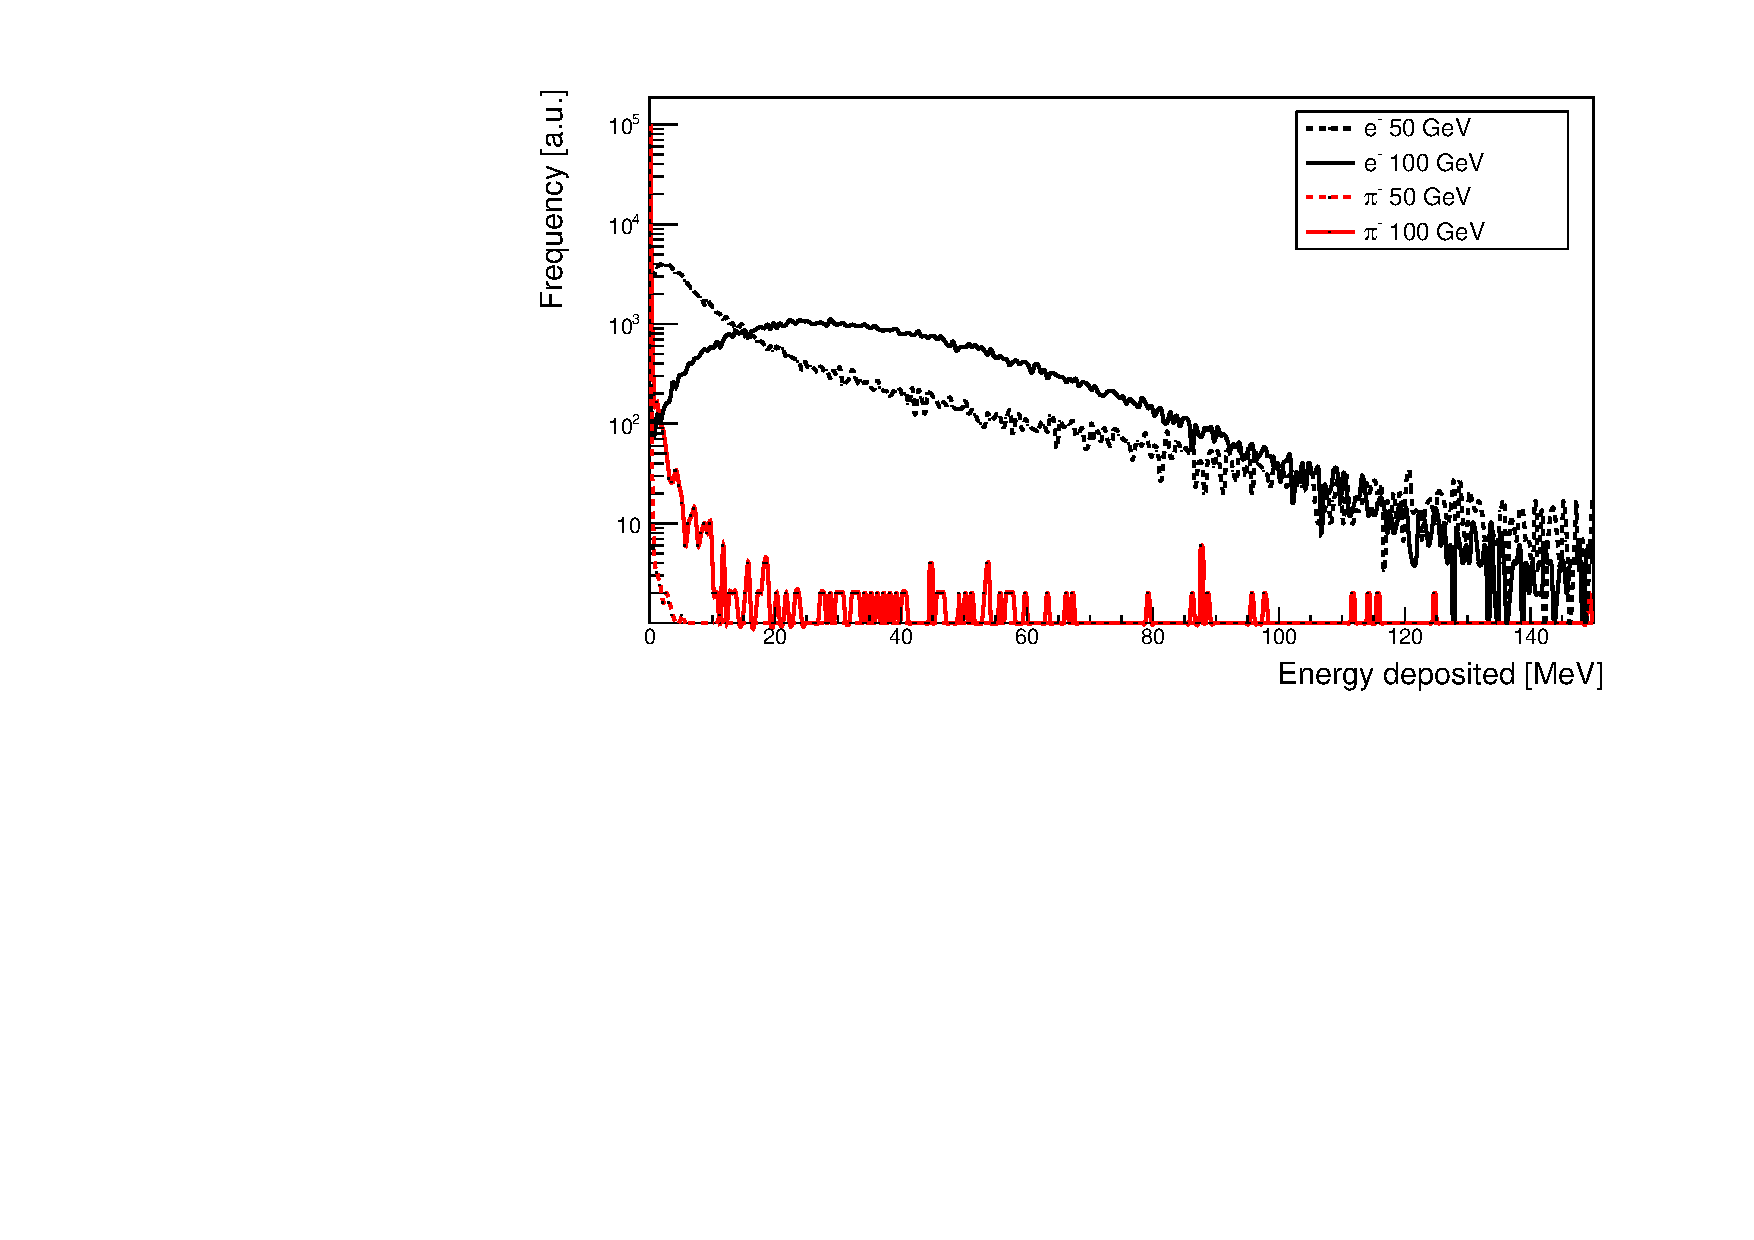
\includegraphics[width=1.\textwidth]{\pdirthree/comp_spectra.pdf}
\caption[SR spectrum for different energy detected in the SRD]{Result of the Geant 4 simulation for the energy detected by the SR detector for 50/100 GeV e$^-$(black dashed/solid line) and 50/100 GeV $\pi^-$ (red dashed/solid line).}
\label{fig:SRspectrum}
\end{figure}

The SRD detector was tested during the NA64 test beam run in July 2016. The two BGO rows are parallel to the primary beam direction as shown in Fig.\ref{fig:newgeo}. The dipole magnets installed in series produce a total integrated magnetic field of 7 T$\cdot$m \cite{Banerjee:2016tad} resulting in a nominal displacement for the incoming electrons at the SRD/ECAL positions of 31/34 cm from the undeflected beam axis. The SRD was placed between the undeflected and the deflected beam axis at a distance of approximately 9 cm from both (Fig.\ref{fig:newgeo}). This separation minimises the possibility for Bremsstrahlung photons and neutral particles produced by interactions of the beam particle with materials upstream (vacuum windows, collimators, trackers...) and for particles in the beam halo (most of the beam used in the experiment was constrained in a circular region with diameter 2 cm) to hit the SRD. In fact, such interactions result in the saturation of the SRD with a significant loss of efficiency due to the long decay time of the BGOs.

%The expected Landau distribution of energy deposits was fit to the data to find the mean peak position to extract the calibration constant. 

The two crystals facing the beam (labeled 3 and 7 in Fig. \ref{fig:newgeo}) detect most of the energy emitted by synchrotron radiation. We will refer to those as SRD BGOs from now on. The remaining six crystals are used to detect events with high energy deposition in the SRD. In particular the last two crystals of each row (labeled 0 and 4 in Fig. \ref{fig:newgeo}) detect some energy only in the case of very energetic Bremsstrahlung events and thus can be used as a veto (see Fig.\ref{fig:newgeo}). The six crystals after the SRD BGOs act also as a shield from backscattering particles coming from the ECAL suppressing pions by an additional order of magnitude. Finally in this geometry it is possible to use the coincidence of the two SRD BGO crystals to improve the tagging of synchrotron photons by rejecting knock-on electrons produced by incoming pions. In fact synchrotron radiation has a homogenous spectrum in the whole arc described by the primary and deflected beam and thus a signal is detected in both SRD BGOs. On the contrary, electrons generated by a $\pi^-$ undergoing ionisation will mostly leave energy only in a single crystal as illustrated in Fig. \ref{fig:newgeo}. 
With the requirement of detecting in both SRD BGOs an energy deposition above a 1 MeV the suppression factor is improved up to a level of $10^{-5}$.



\begin{figure}[htb!]
  \centering
  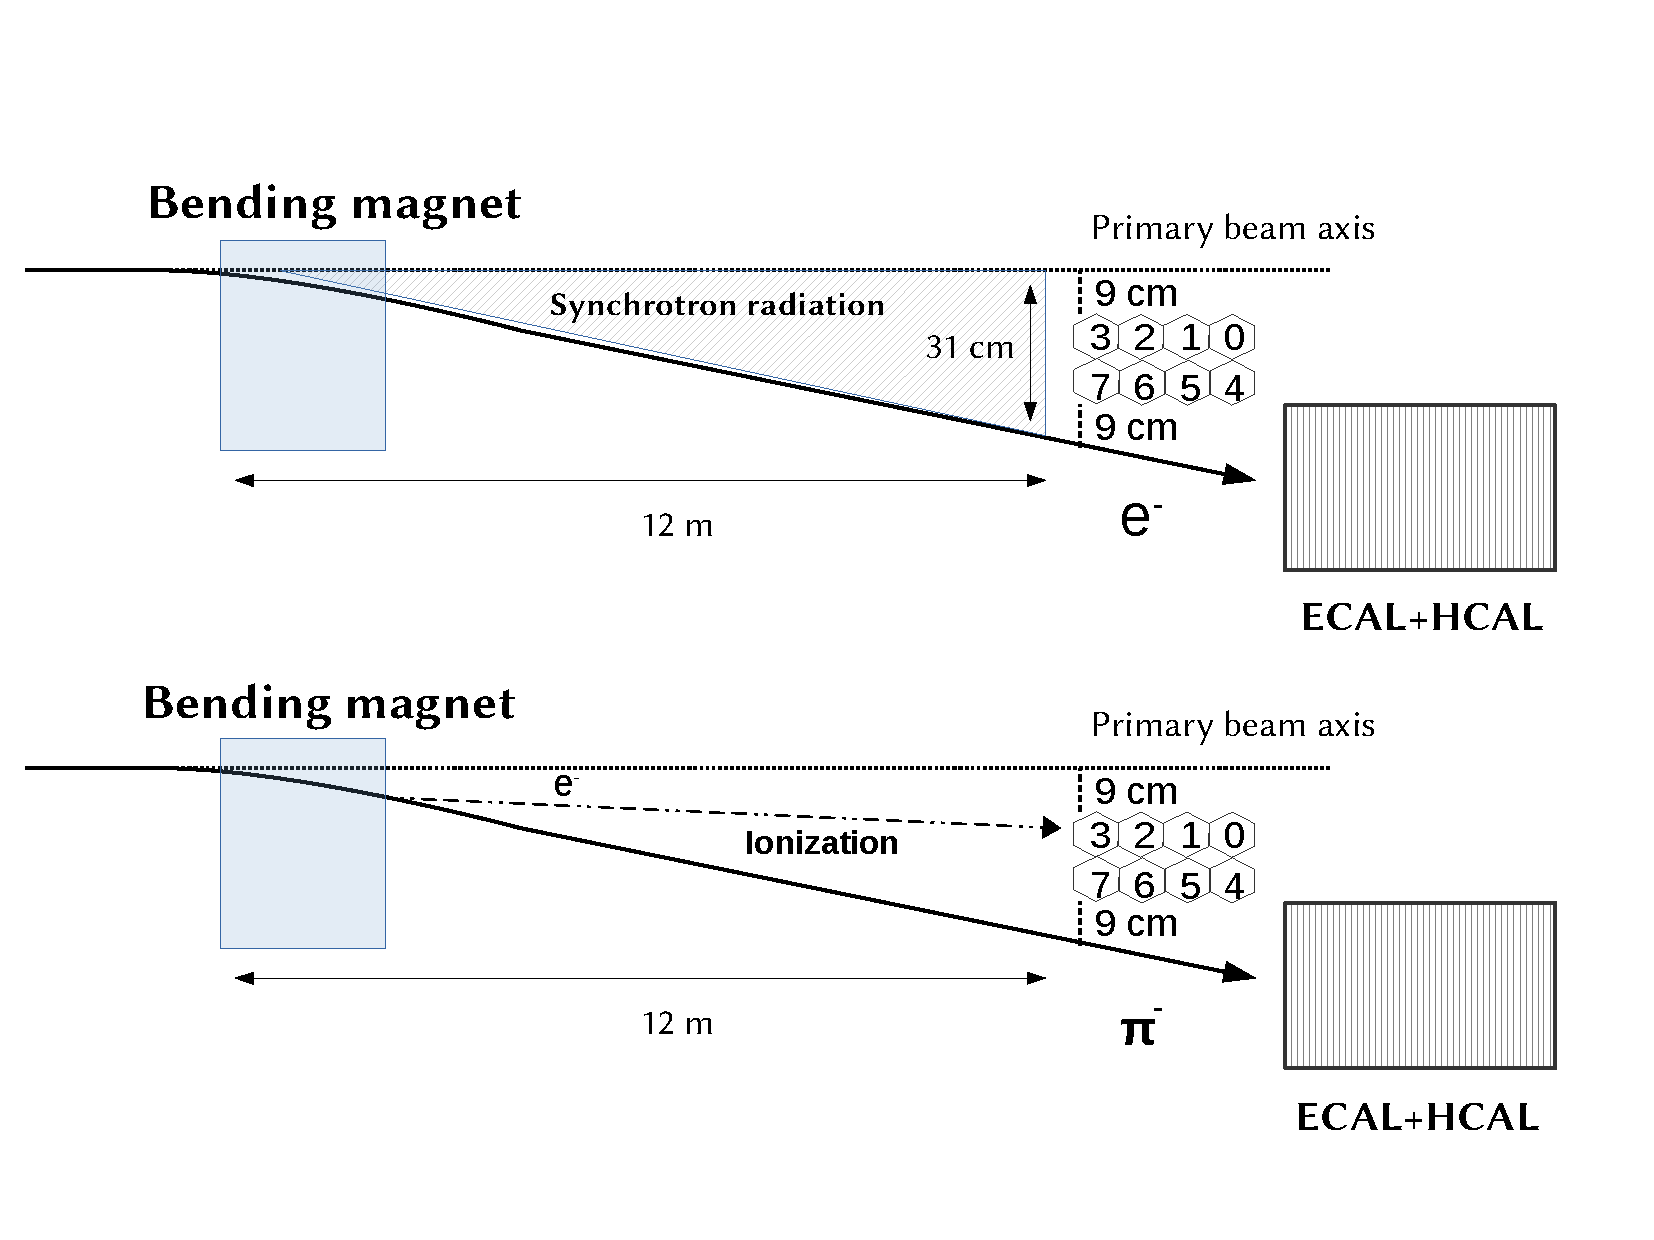
\includegraphics[width=.9\textwidth]{\pdirthree/sketch.pdf}
  \caption[Geometry of the BGO crystals]{Geometry of the BGO crystals. Crystals 7,3 (SRD BGO) collect most of the synchrotron radiation spectrum. Crystals 4,0 (VETO BGO) on the other hand are effected only in case of a high energy event and are thus used as a veto. The remaining crystals serve as a shield for the SRD from backscattering particles coming from the ECAL. Top: illustration of event leaving a SR signal in the SRD. Bottom: illustration of a SR- like signal in the SRD for a knock-on electron produced by pions.}
\label{fig:newgeo}
\end{figure}

Data with a 100 GeV $\pi^-$ beam were taken to have a direct measurement of the suppression factor achievable through synchrotron radiation measurements. The beam intensity was 5.3$\times 10^4$ particles per spill. The trigger was given by the coincidence of the three plastic scintillator counters (S1, S2 and S3 shown in Fig.\ref{fig:setup-invis-2018}). The additional requirement of an energy deposition below 60 GeV in the ECAL was applied in order to select an almost pure $\pi^-$ sample of $\sim 10^5$ collected events. The probability for electrons to punch through the 40 radiation lengths of the ECAL was estimated to be at a level of $10^{-12}$ \cite{Banerjee:2016tad}. 

For the 100 GeV electron beam run, a total of 220 spills were recorded with an intensity of 3.4$\times 10^5$/spill. 
The same trigger used in the pion run was used for the electron data.
In this case though, in order to reduce the pion contamination which is at a level of few \% and obtain a pure sample of electrons-only events with a total energy deposition in ECAL + HCAL above 90 GeV but with less than 20 GeV energy in the HCAL were used.  


The energy spectra recorded by the SRD BGO with electrons and pions are shown in Fig.\ref{fig:comp_spectra}. The SR spectra obtained with the electron beam are used to perform the BGO calibration by comparison with the simulation. With this method a very good agreement of data and MC is achieved (see plot on the left of Fig.\ref{fig:comp_spectra}). As a cross check, using the obtained calibration constants, the data from the pion beam impinging directly on the SRD are fitted with a Landau distribution. The obtained peak position of 60 MeV is in good agreement with the prediction of the MC. 

Time coincidence of signals above the energy threshold of 1 MeV from both SRD counters is required and high energy Bremsstrahlung events are removed using the veto BGO.
The suppression of synchrotron radiation emission detected for pions compared to electrons is clearly visible by comparing the two plots. For the electron spectrum, a 1\% pileup beam events have been added to the simulation as predicted for the given spill intensity and with the known decay time of BGOs.  Both spectra are in very good agreement with the simulation.

\begin{figure}[htb!]
  \centering
  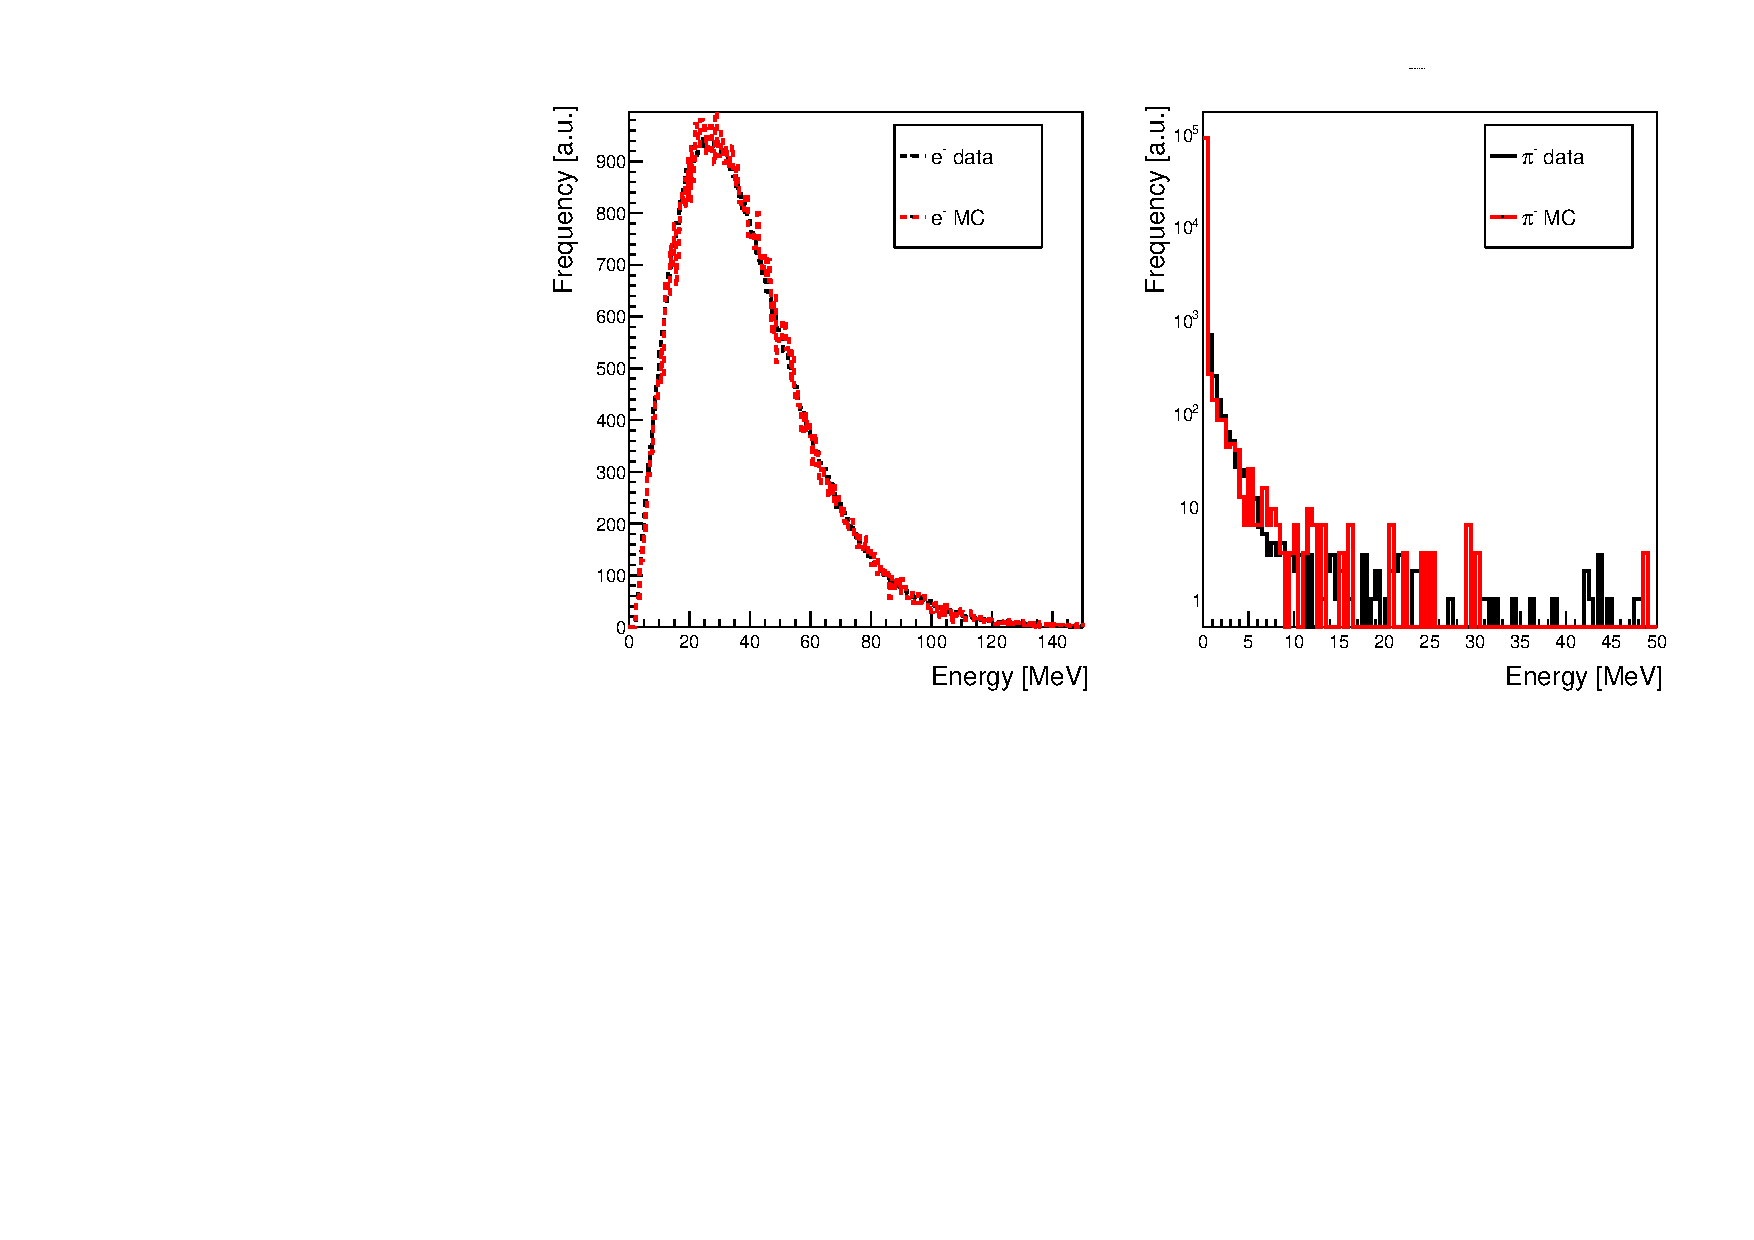
\includegraphics[width=1.\textwidth]{\pdirthree/spectra_tot.pdf}
  \caption[SRD comparison between data and MC]{Comparison between data and simulation (MC) of the synchrotron radiation spectrum detected for 100 GeV electrons (left) and pions (right). }
  \label{fig:comp_spectra}
\end{figure} 

\begin{figure}[htb!]
  \centering
  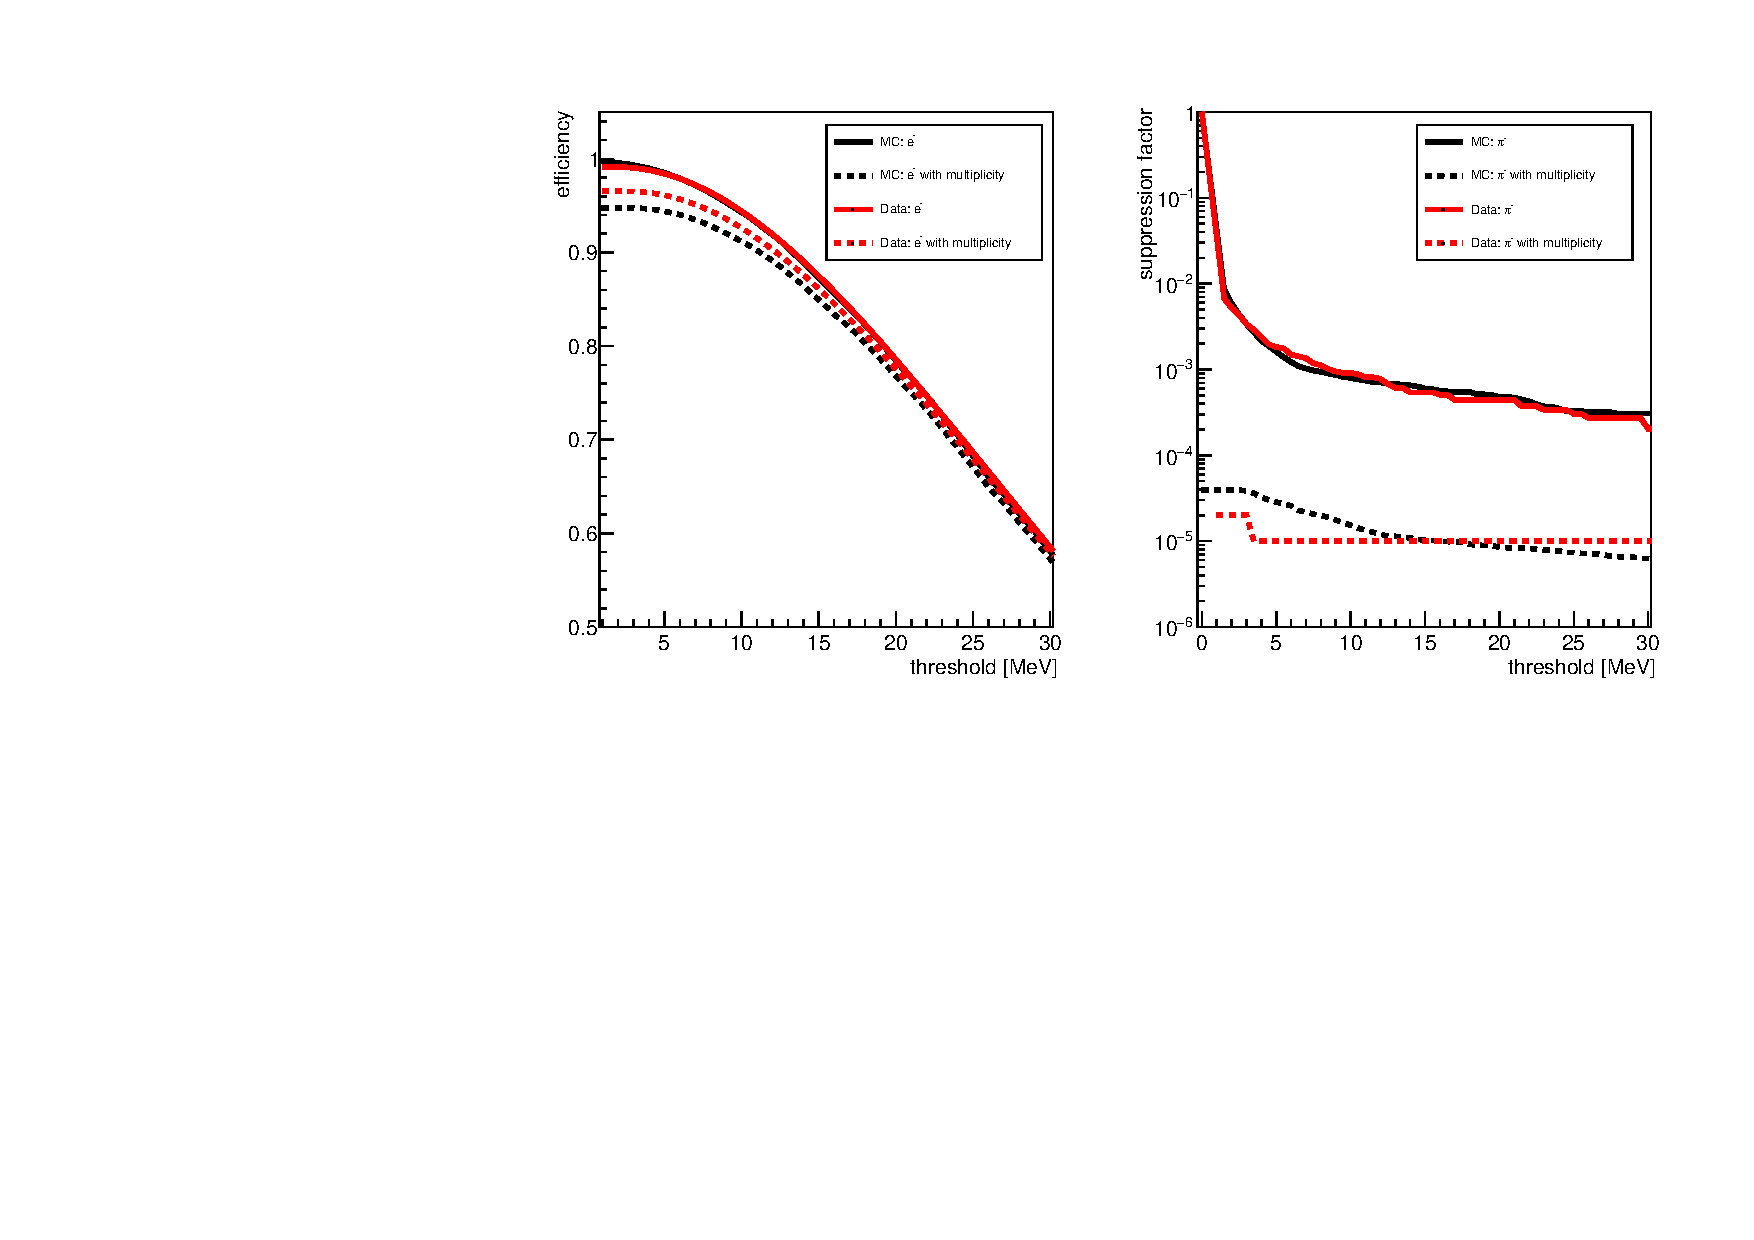
\includegraphics[width=1.\textwidth]{\pdirthree/sup_mult.pdf}
  \caption[efficiency and rejection power of the SRD cut]{Left: Comparison between data and simulation (MC) for electrons of the efficiency as a function of threshold set on the total energy deposited in the SRD BGO and for the requirement that this is deposited in each single crystal (multiplicity). Right: Comparison between data and simulation for pions and electrons of the suppression factor as a function of the threshold set on the total energy deposited in the SRD BGO and for the multiplicity requirement.}
  \label{fig:sup_mult}
\end{figure}

The efficiency for the electrons and the suppression factor for the pions are plotted in Fig. \ref{fig:sup_mult} as a function of the threshold on the energy deposited in the SRD. We distinguish between two cases:
\begin{enumerate}
\item The threshold is set on the total energy deposited in the SRD.
\item Both SRD signals have to be in-time and above the threshold of 1 MeV (multiplicity requirement).
\end{enumerate}
One can see that applying the criterion 2) the efficiency only decreases slightly compared to 1), while the suppression factor for pions is dramatically increased (by two orders of magnitude) with the requirement of having the two BGOs in coincidence.
This can be understood because the SR-like signal generated from secondary electron will leave a signal only in one of the two BGOs while the SR from electrons is spread out uniformly as explained above. 
This is also nicely evidenced by Tab. \ref{tab:hits} where the fraction of events with different hit multiplicity in the SRD BGO for both pion and electron runs are reported.

\begin{table}[hbt!]
\begin{center}
\begin{tabular}{cccc}
Events hit multiplicity  (\%) & 0 BGO  & 1 BGO & 2 BGOs\\
\hline
Pions & $98.77$ & $1.21$ & $1.4\times10^{-3}$  \\
Electrons & $2.4\times10^{-1}$  & $2.60$ & $97.37$ \\
\end{tabular}
\end{center}
\caption[Fraction of pion and electron events for different hit multiplicity in the SRD from the data]{Fraction of pion and electron events for different hit multiplicity in the SRD from the data.}
\label{tab:hits}

\end{table}

\subsection{Hadron rejection using electromagnetic shower profile}
\label{ch3:sec:bkg-ecal-profile}

The critical task of rejecting the hadron contamination in the H4 beam
is currently performed by the SRD (synchrotron radiation detector) and
the detectors placed behind the ECAL (namely the VETO and the HCAL
modules). In the following note we present a method to exploit the
information from the energy deposition in the ECAL cells to separate
events that produce an electromagnetic shower from the one inducing an
hadronic one to further increase the purity of our sample.
\\
\\
The analysis is done by following the strategy proposed by Alexandre
Toropin of using the extrapolated line obtained from the last two
MicroMegas planes to extract the hit point of the particle on the
ECAL. A shower profile database can be built by correlating the hit
position (x,y) on the ECAL with the fraction of energy deposited in
each ECAL cell. From this database a predicted value of energy
deposition in each ECAL cell can be extracted and compared to the one
of each single event. The compatibility between the predicted profile
and the measured one can be tested using the
$\chi^2$-distribution. Namely the following equation is used:

\begin{equation}
  \chi^2 = \sum^{9,36}_i \left(\frac{E_{pred}^i(x_{hit},y_{hit})-E_{mes}^i}{\sigma^{i}_{pred}(x_{hit},y_{hit})}\right)^2
  \label{eqn:chi}
\end{equation}


\begin{description}
\item[$E_{pred}^i$]: is the energy predicted by the profile of cell
  $i$
\item[$E_{mes}^i$]: is the energy measured in the cell $i$
\item[$x_{hit},y_{hit}$]: coordinates of the hit position of the
  particle in the ECAL plane
\item [$\sigma^{i}_{pred}$]: error estimated for the predicted energy
  in cell $i$
\end{description}


Two different summation indexes are used for the two different cases
where only the cells surrounding the central one hit by the beam are
used for the test (total of 9 cells) and the case where all the cells
are used (total of 36, see Fig.\ref{fig:ecal_example}).
\\
\\
As correctly stated by Alexandre Toropin, assuming axial symmetry for
the shower can reduce the redundancy of the profiles by considering
only the region ($0 \leq x_{hit} \leq d/2$ $\bigwedge$
$0 \leq y_{hit} \leq d/2$) where $d$ is the dimension of one ECAL
cell. Since however the time required to create the database and
perform the analysis does not change significantly under this
assumptions we choose to record the behaviour of the electromagnetic
shower in the whole cell in order to reduce possible asymmetries
produced by the inhomogeneities of the ECAL.

\begin{figure}[h!]
  \begin{center}
    \includegraphics[scale=0.47,page=4]{\pdirthree/ecal_example.pdf}
  \end{center}
  \caption[ECAL sketch]{sketch of the 36 cells of the ECAL. The central cell 3X3
    were the beam is directed is plotted in red, while the cells
    surrounding it are plotted in green. On the bottom-right an
    example of how a profile for a cell looks like in the MC.}
  \label{fig:ecal_example}
\end{figure}


 
\subsubsection{Construction of the profiles}
\label{ch3:sec:make_profile}

A shower profile database can be understood as an $N\times N$ matrix
where each entry represents a portion of the ECAL cell of dimension
$d_x \times d_y$. Each entry of the matrix contains the mean value of
energy deposited in the cell when the incoming particle hits the
portion of the ECAL plane described by that entry. In order to also
account for the deviation that such shower can have as function of the
hitting point one would need a second matrix to encode such
information. To build such database the root function was used
TProfile2D, this object has the advantage to be highly flexible and
allows compact codes due to its integrated function. The complete
documentation of this object can be found in Ref.\cite{root-tprofile}.
\\
\\
The main parameters that play a role in the construction of the shower
profiles are the dimensions of the area that is covered by the
TProfile2D, and the dimensions $d_x \times d_y$ that each bin has,
which represents the minimal distance between two hit points that can
be resolved by the database.  The total dimension that the profile
should have can be trivially set to be equal to the ones of one ECAL
cell (38.2$\times$38.2 mm, see \cite{na64-detectors}) since our cuts
already requires the majority of the shower to be contained in the
cell aligned with the beam spot. The problem of the bin dimension is
more subtle: due to the shower symmetry there is no particular reason
to set $d_x \neq d_y$ the precise dimensions of the bin must be a
compromise between having a large bin that allows good statistic and a
small bin that allows enough precision. The large sample of electrons
collected in NA64 typically allows good statistic for each bin even
when their dimension is below 1 mm, however defining a bin smaller
than the accuracy that we are able to achieve in the extrapolation of
the MicroMegas line to the ECAL should be avoided. This error can be
derived analytically to be:
\begin{equation}
  \sigma_{ECALxy} = \sigma_{mm}\sqrt{1+2t^2}
  \label{eqn:MMerror}
\end{equation}

\begin{equation}
  t = \frac{Z_{ECAL}-Z_{MM4}}{Z_{MM4}-Z_{MM3}}
  \label{eqn:T}
\end{equation}

where:
\begin{description}
\item[$\sigma_{ECALxy}$]: is the error of the hit position
  extrapolated to the ECAL in the xy-plane
\item[$\sigma_{mm}$]: is the resolution of the hit position in each
  MicroMegas
\item[$Z_{MMi}$]: is the position in the Z-axis of the MicroMegas
  Nr. i
\item[$Z_{ECAL}$]: is the position in the Z-axis of the ECAL plane
\end{description}


This results in a resolution of $\sim$130 $\mu$m for our setup. A more
complicate expression was considered to take into account possible
misinformation in the exact position of the detectors. While the exact
entrance angle of the particle was checked to have small effects on
$\sigma_{ECALxy}$, assuming some error on the exact position of the
detectors increases the error by a factor 2-4 for values around 1-2
cm. The work presented in this note was performed using a TProfile2D
with bin size of 0.34 mm which accounts for such uncertainties.
\\
\\
Only calibration runs without physical trigger were used to produce
the profiles in order to have a sample of electrons, cuts were applied
to
reject the contamination caused by the hadrons in the beam and out-of-time energy events. \\
The following criteria were applied for the profiles tested in this
note:

\begin{itemize}
\item single cluster in each MicroMegas
\item energy larger than 1 MeV and smaller than 70 MeV in each SRD
  plane
\item coincidence of $\sim$1 ns between timing in cell (3,3) of ECAL
  and mastertime
\item pedestal fluctuation less than 10 ADC in cell (3,3) and each of
  the surrounding cells
\end{itemize}

The code used to produce the profiles
has been integrated in the official reconstruction library of NA64 and can
be easily customized to produce profiles with different cuts.
\\
\\
The production of the database is done for the events
selected by computing the hit point of the incoming particle in cell
3x3 and updating the value of the corresponding bin in each of the 36
TProfile2D representing each cell. The specific value filled is the
percentage of energy deposited in the cell, i.e. $100 \times E^i/E^{tot}$.
The error over this value is automatically computed by the TProfile2D.
\section{$\chi^2$ computation}
\label{ch3:sec:chi2-comp}

The algorithm for the $\chi^2$ computation works as follows:
\begin{enumerate}
\item The values of the xy coordinates of the hitting point of the
  particle are computed by extrapolating to the ECAL position the line
  passing through the hit point of the last two MicroMegas planes.
\item The predicted values $E_{pred}^i$,$\sigma^{i}_{pred}$ are read from the TProfile2D in
  the corresponding bin
\item The values $E_{mes}^i$ are computed normalizing the energy $E^i$
  of each cell to the total energy measured in the ECAL.
\item The value of $\chi^2$ is calculated using Eq.\ref{eqn:chi} and is
  normalized to the number of cells considered.
\end{enumerate}

\section{Results}
\label{ch3:sec:chi2-result}

A database was produced using the method described in
Sec.\ref{ch3:sec:make_profile} and using the calibration runs 2363, 2182,
2410, 2406, 2438. A complete description of such runs can be found in
\cite{na64-runs}. To test the rejection power and the efficiency of the
method the algorithm described above was used for 3 type of runs:
\begin{enumerate}
\item the calibration run 2363 to test the efficiency of the method
\item the hadron run 2204 to test the suppression factor of the method
\item the physical run 2441 to test the effect of the cut on the ECAL
  vs HCAL plot on a run with physical trigger at high intensity.
\end{enumerate}

The comparison of the normalized $\chi^2$-distribution between
electron calibration run and hadron run using information from all 36
cells is shown in Fig.\ref{fig:chi2}. Note that electrons reproduce
the expected shape of a $\chi^2$-distribution while for hadrons we
observe a displaced one incompatible with the one produced by
electrons.  The rejection and efficiency of a cut
$\chi^2 < \chi^2_{cut}$ are shown in detail in Fig.\ref{fig:eff}. For
a benchmark $\chi^2$-cut of 2 the efficiency calculated in run 2363
was $\sim 0.94$ with a rejection factor of $1.2\times 10^{-3}$
calculated from the hadron run 2204. These values as well as the ones
presented in Fig.\ref{fig:eff} are computed by looking at the total
number of events passing the cut and do not account for the impurities
in the beam.
\\
\\
Using information coming only from the 9 central
cells (Fig.\ref{fig:ecal_example}) appears to shift the distribution
to the left and reduce its spread ( Fig.\ref{fig:chi}) due to the
smaller number of degrees of freedom, the two methods have overall
comparable efficiency as can be seen in Fig.\ref{fig:eff} but smaller
rejection power when a typical cut is applied.  For the considered
benchmark cut of $\chi^2_{cut}=$2, the efficiency measured using only
central cells was of $\sim 0.93$\ and a rejection factor of
$3.1\times 10^{-3}$.


\begin{figure}[h!]
  \begin{center}
    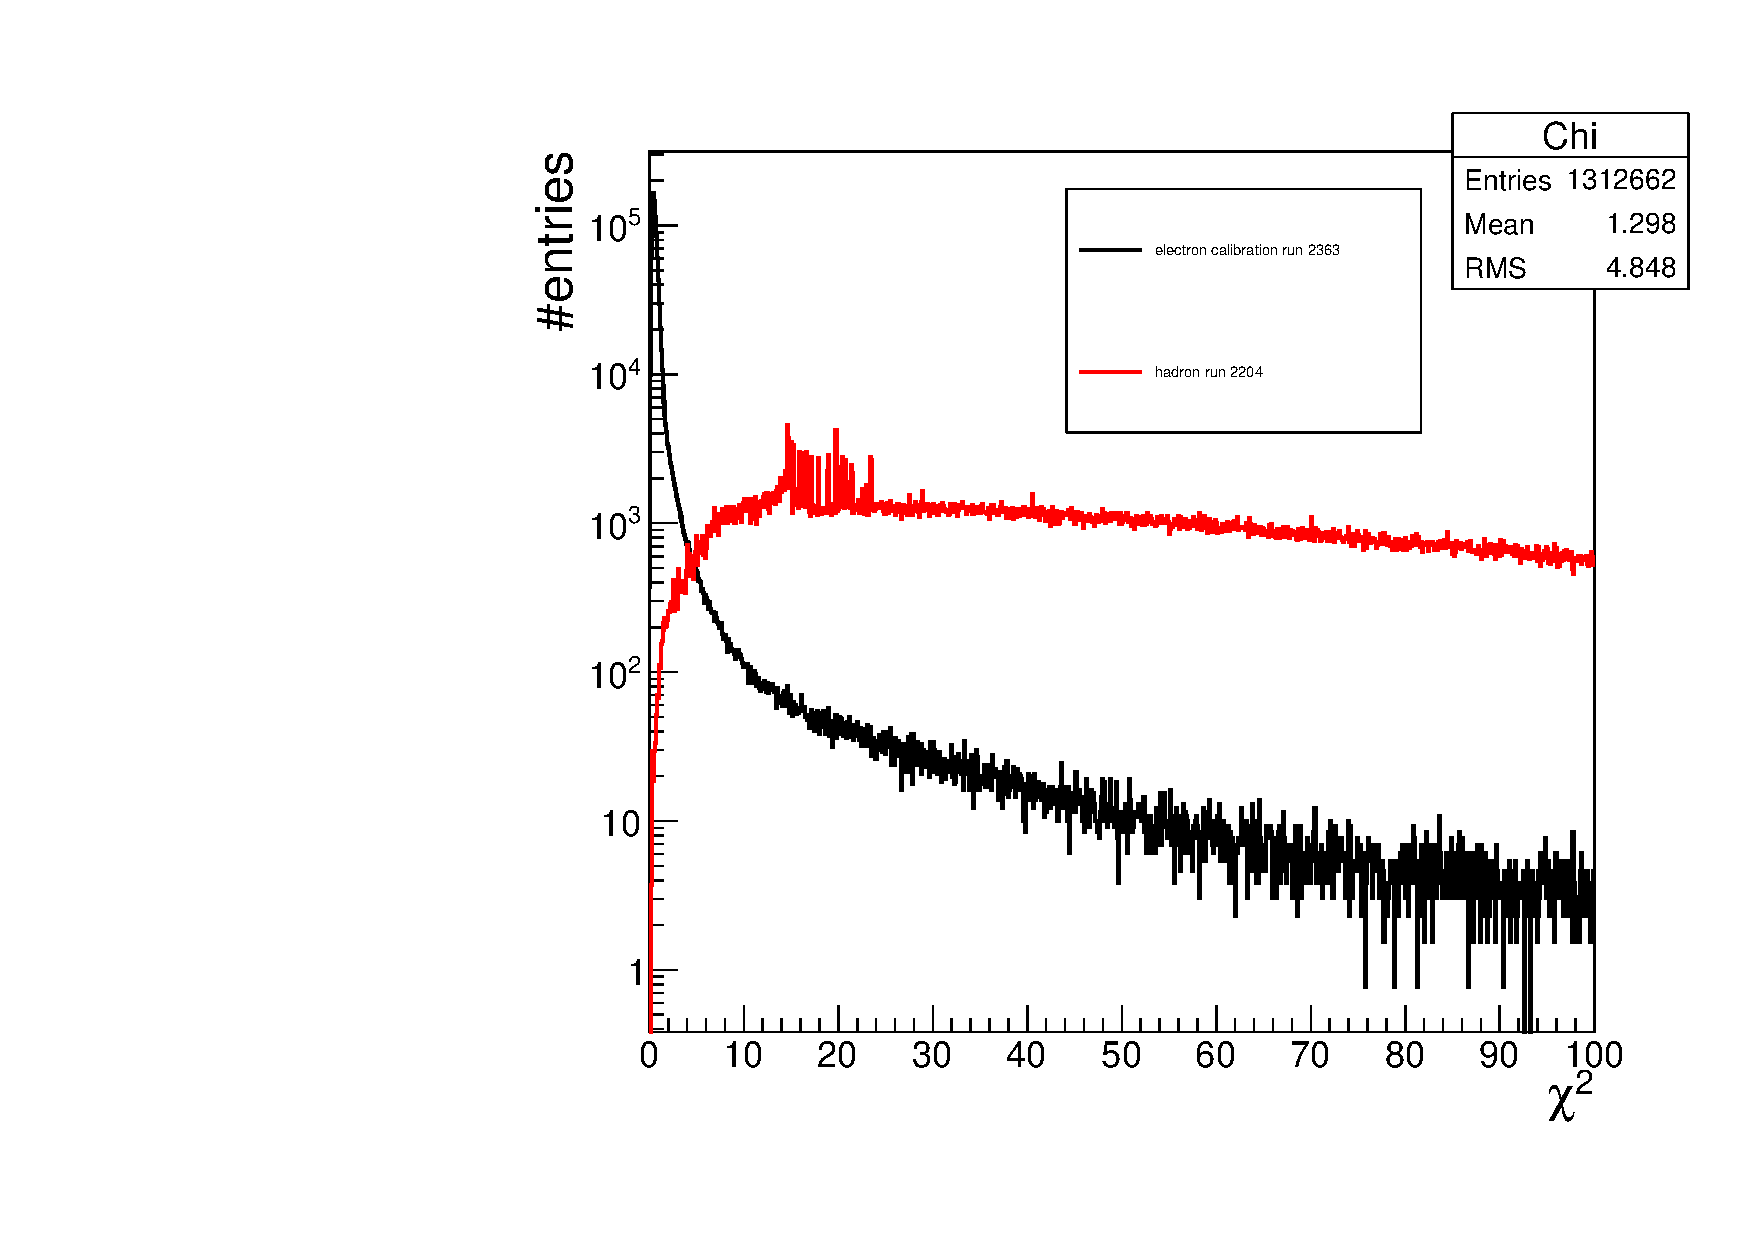
\includegraphics[width=0.95\textwidth,height=0.8\textwidth]{\pdirthree/chi_comp.pdf}
  \end{center}
  \caption[comparison between $\chi^2$ distribution, electron and hadron calibration run]{comparison between $\chi^2$ distribution generated from the
    calibration run 2363 and the hadron run 2204.}
  \label{fig:chi2}
\end{figure}

\begin{figure}[h!]
  \begin{center}
    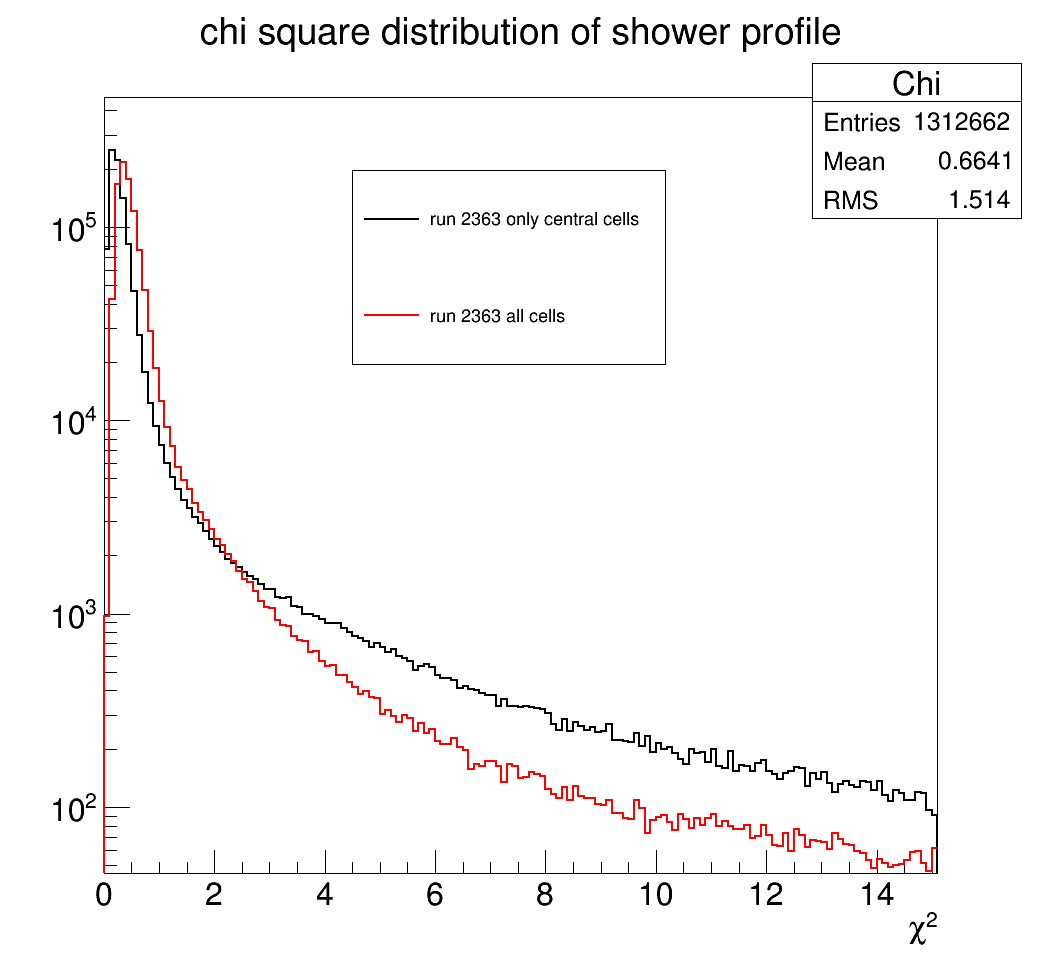
\includegraphics[width=0.95\textwidth,height=0.8\textwidth]{\pdirthree/plot_comp_cells.png}
  \end{center}
  \caption[comparison between $\chi^2$ distribution for different ECAL configurations]{comparison between $\chi^2$ distribution generated from run
    2363 considering only central cells (black) and considering all 36
    cells (red).}
  \label{fig:chi}
\end{figure}

\begin{figure}[h!]
  \begin{center}
    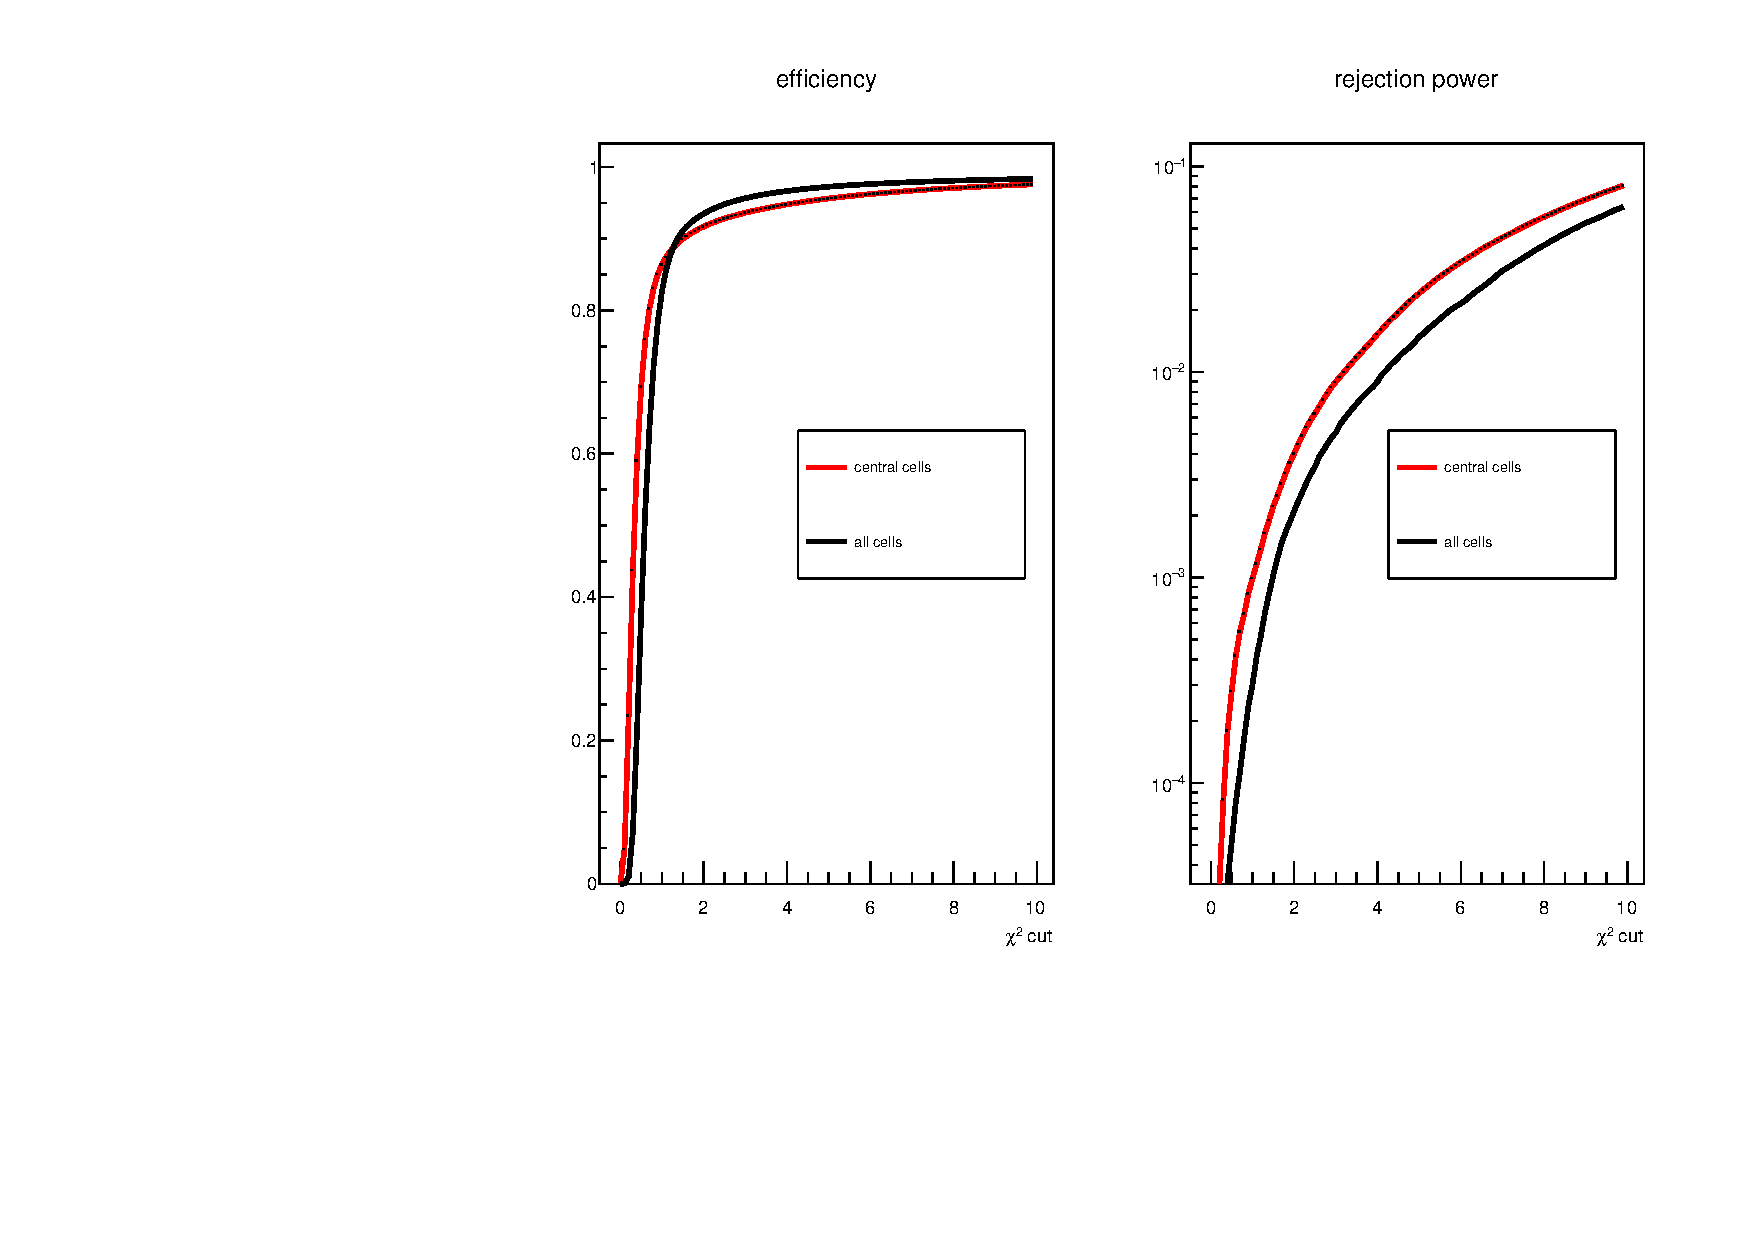
\includegraphics[width=0.95\textwidth,height=0.6\textwidth]{\pdirthree/eff.pdf}
  \end{center}
  \caption[fraction of events passing the $\chi^2$ cut]{fraction of events passing the cut $\chi^2 < \chi^2_{cut}$
    for the calibration run 2363 (left plot) and for the hadron run
    2204 (right plot).}
  \label{fig:eff}
\end{figure}

\clearpage

Different ECAL vs HCAL plots were produced to study the effect of a
$\chi^2$-cut for the run mentioned above. The one produced with
benchmark cut of $\chi^2 < 2$ are shown in
Fig.\ref{fig:ehcal_test}. The cut is shown to clean the plot in the
way expected from the hadronic activity in all selected runs. Also it
can be seen from the run 2441 that the events involving the di-muon
transition $e^- \to \mu^+\mu^-$ survive the cut for energies larger
than 20 GeV.  This is expected since these events will still involve
an electromagnetic shower truncated in the moment the transition
happens. Since a possible signal from a Dark Photon would behave
similarly this suggest that the cut won't reject the signal provided
that the shower has enough energy. A similar study performed with the
MC (see Sec.\ref{ch3:sec:mc}) reached the same conclusion, however for
very small energies the shower shape will slowly reach the energy
resolution in each cell and the efficiency of the cut will drop
substantially.  The efficiency for low energy improves if only central
cells are selected for the $\chi^2$ calculation since this will reduce
the fluctuation of the single cells not involved in the shower. This
effect is shown in Fig.\ref{fig:ehcal_comp} for the physical run 2441
for a cut of 2 on $\chi^2$.
\\
\\
For low energy particles it is clear that all the shower will be
contained in the cell 3x3. Below this threshold shower analysis can no
longer resolve the type of shower of the event and instead the simple
requirement of the full energy of the event to be detected by the
central cell (3x3) should be used to avoid killing the
signal. Applying a $\chi^2$-cut to a dark photon simulation (see
Sec.\ref{ch3:sec:mc}) suggested that this limit is roughly 5 GeV.  The
left plot in Fig.\ref{fig:ehcal_comp} is compatible with this
estimate.


\newpage
\begin{figure}[h!]
  \begin{center}
    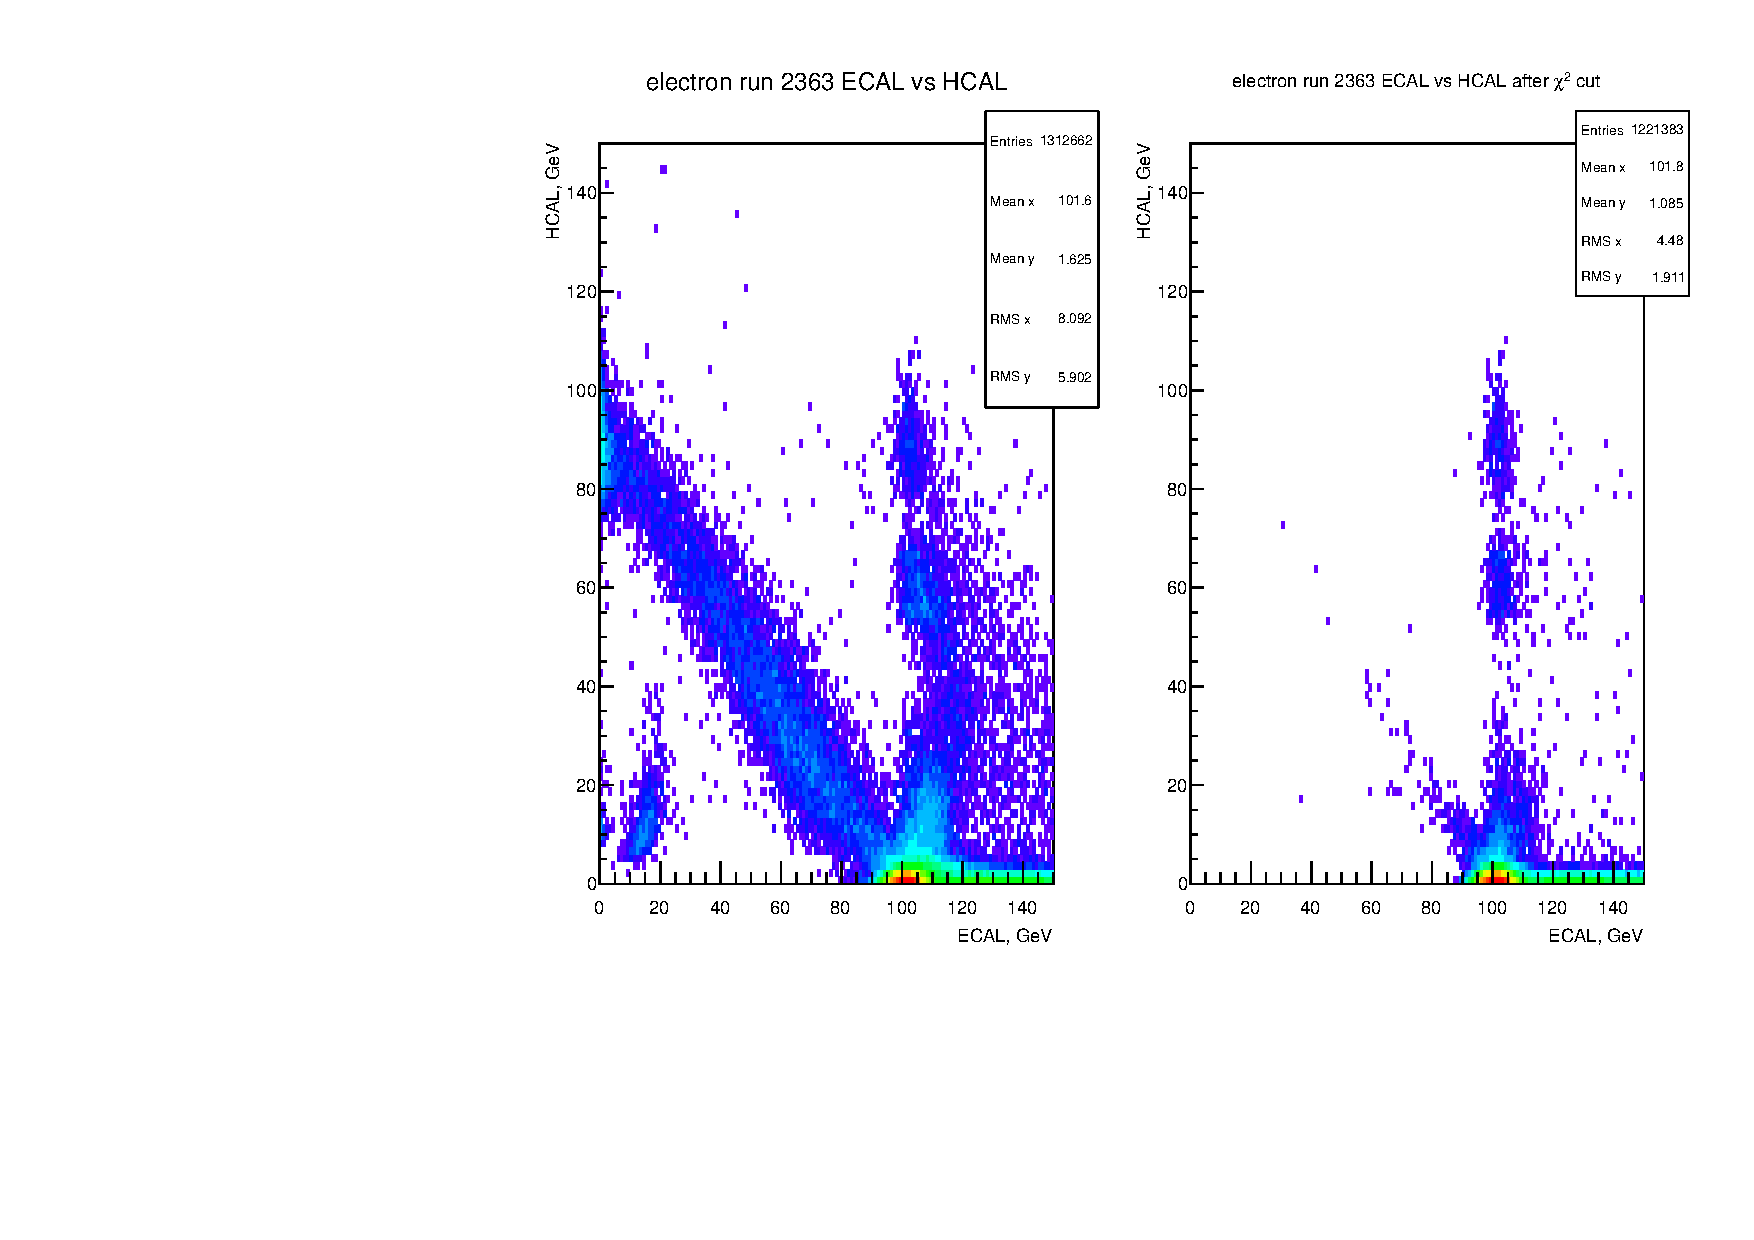
\includegraphics[width=0.95\textwidth,height=0.45\textwidth]{\pdirthree/ehcal_2336_chi.pdf}
    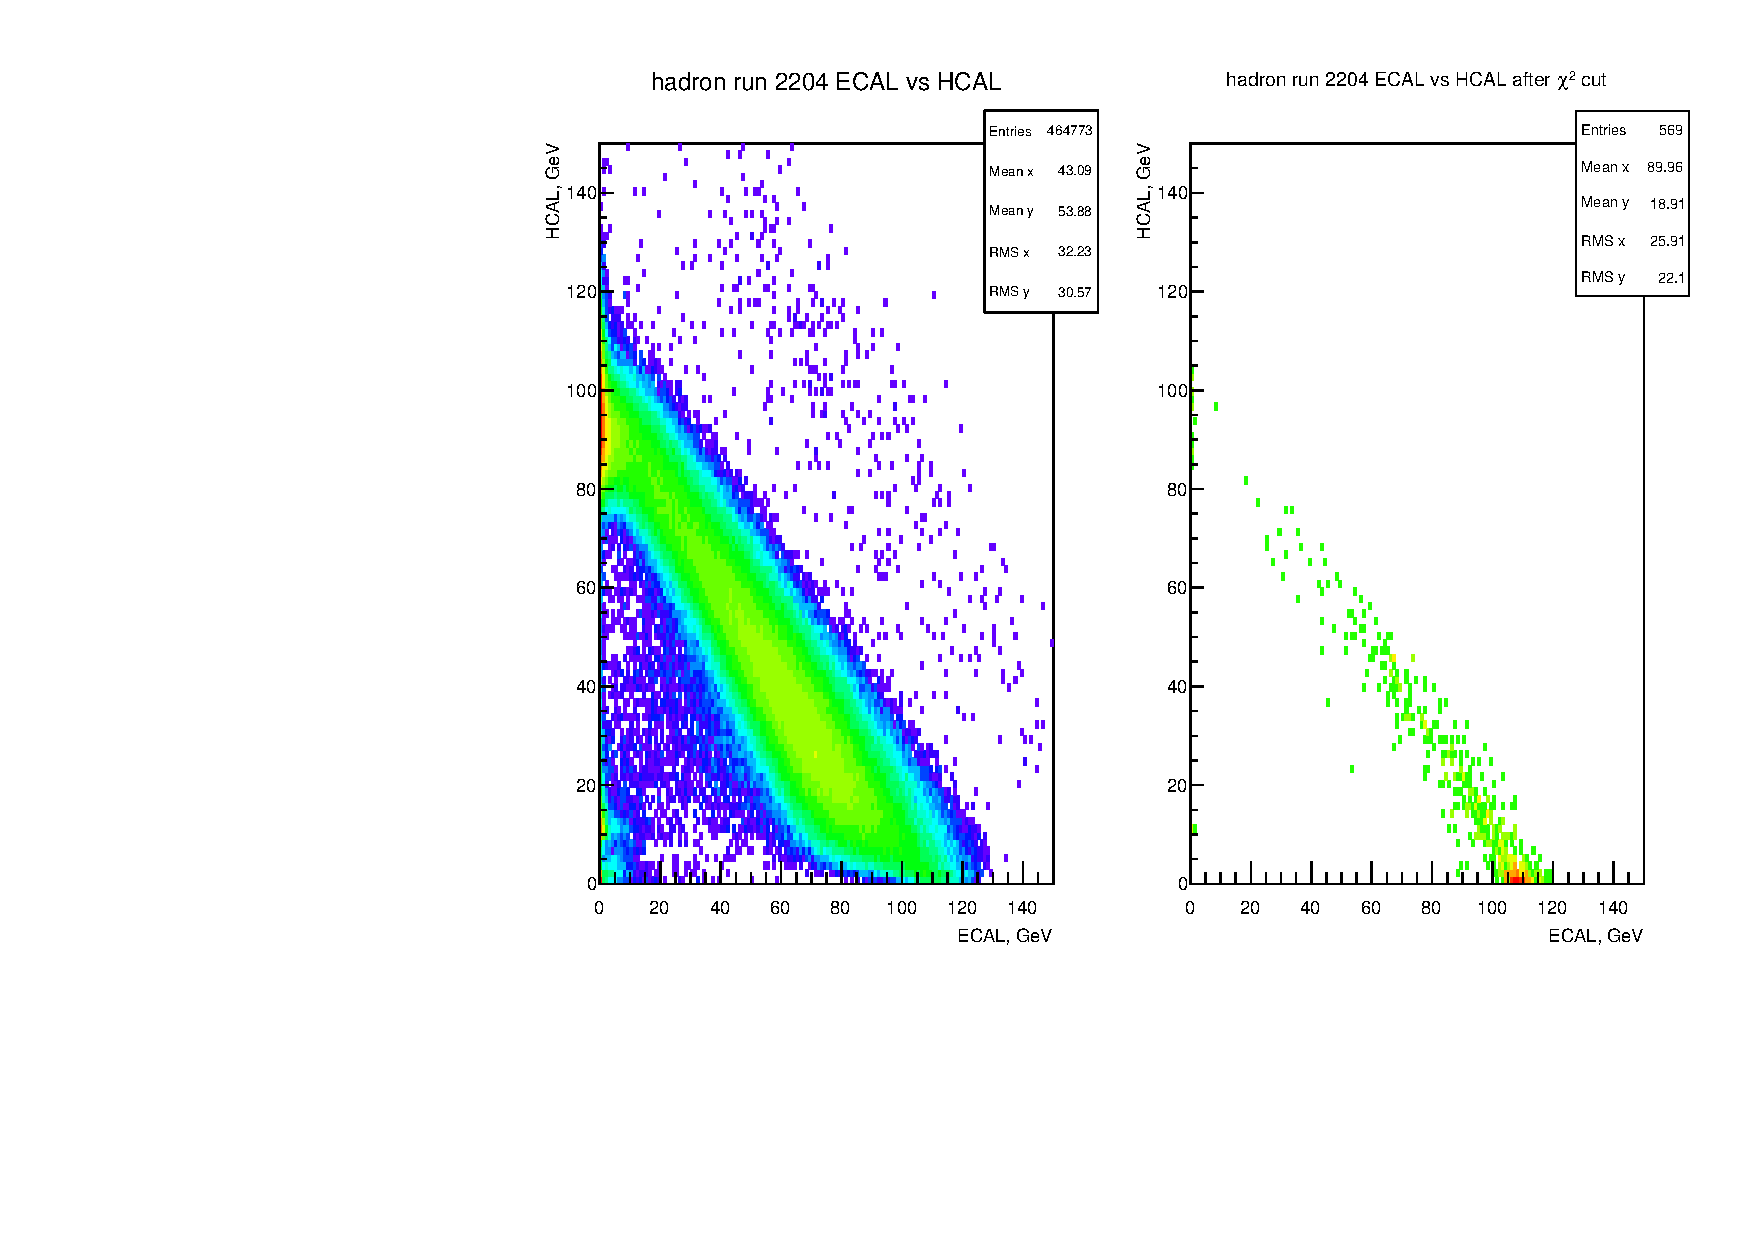
\includegraphics[width=0.95\textwidth,height=0.45\textwidth]{\pdirthree/ehcal_2204_chi.pdf}
    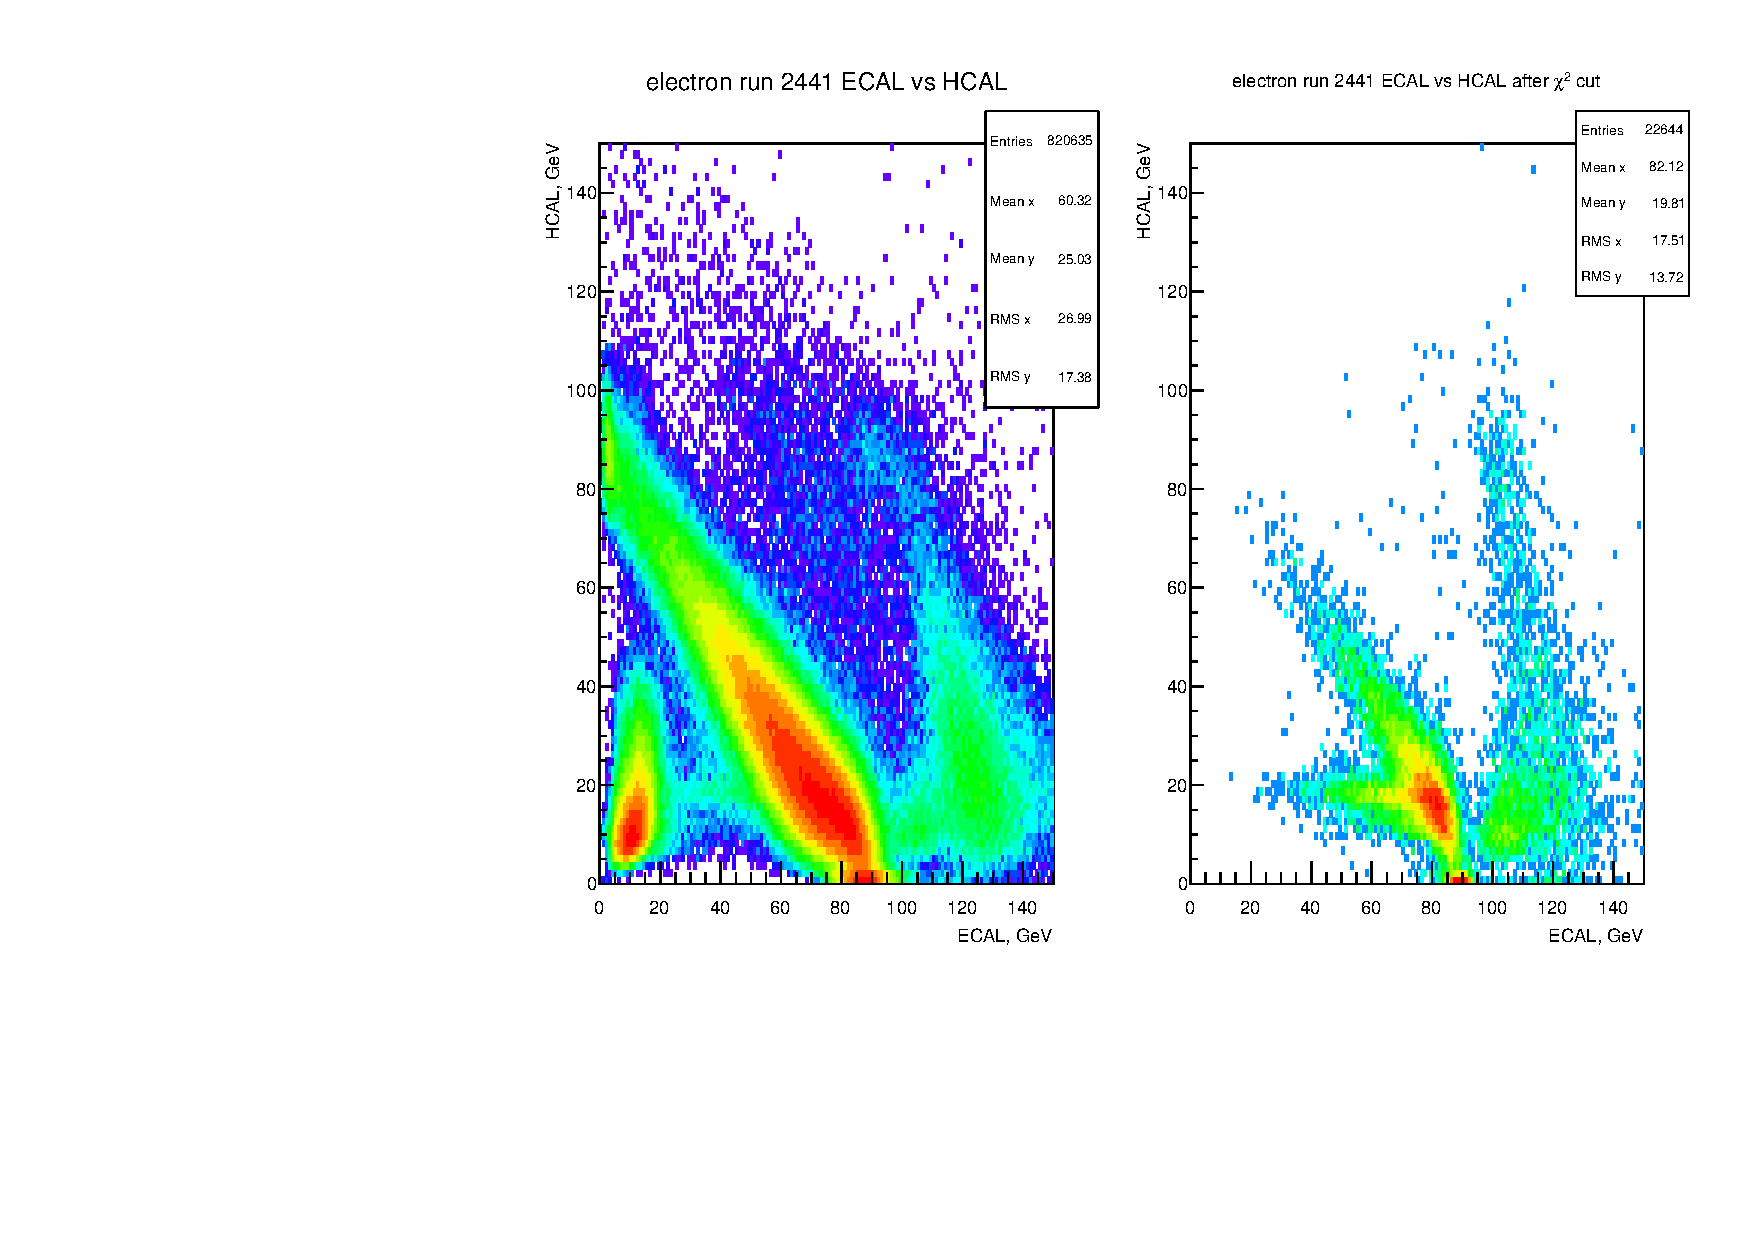
\includegraphics[width=0.95\textwidth,height=0.45\textwidth]{\pdirthree/ehcal_2441_chi.pdf}
  \end{center}
  \caption[ECAL vs HCAL energy deposit after a cut $\chi^2$]{ECAL vs HCAL energy deposit for the total sample (left
    column) and after a cut $\chi^2<2$ (right column) for the
    calibration run 2363 (top), the hadron 2204 run (middle) and the run
    2441 with physical trigger(bottom).}
  \label{fig:ehcal_test}
\end{figure}
\clearpage

\begin{figure}[h!]
  \begin{center}
    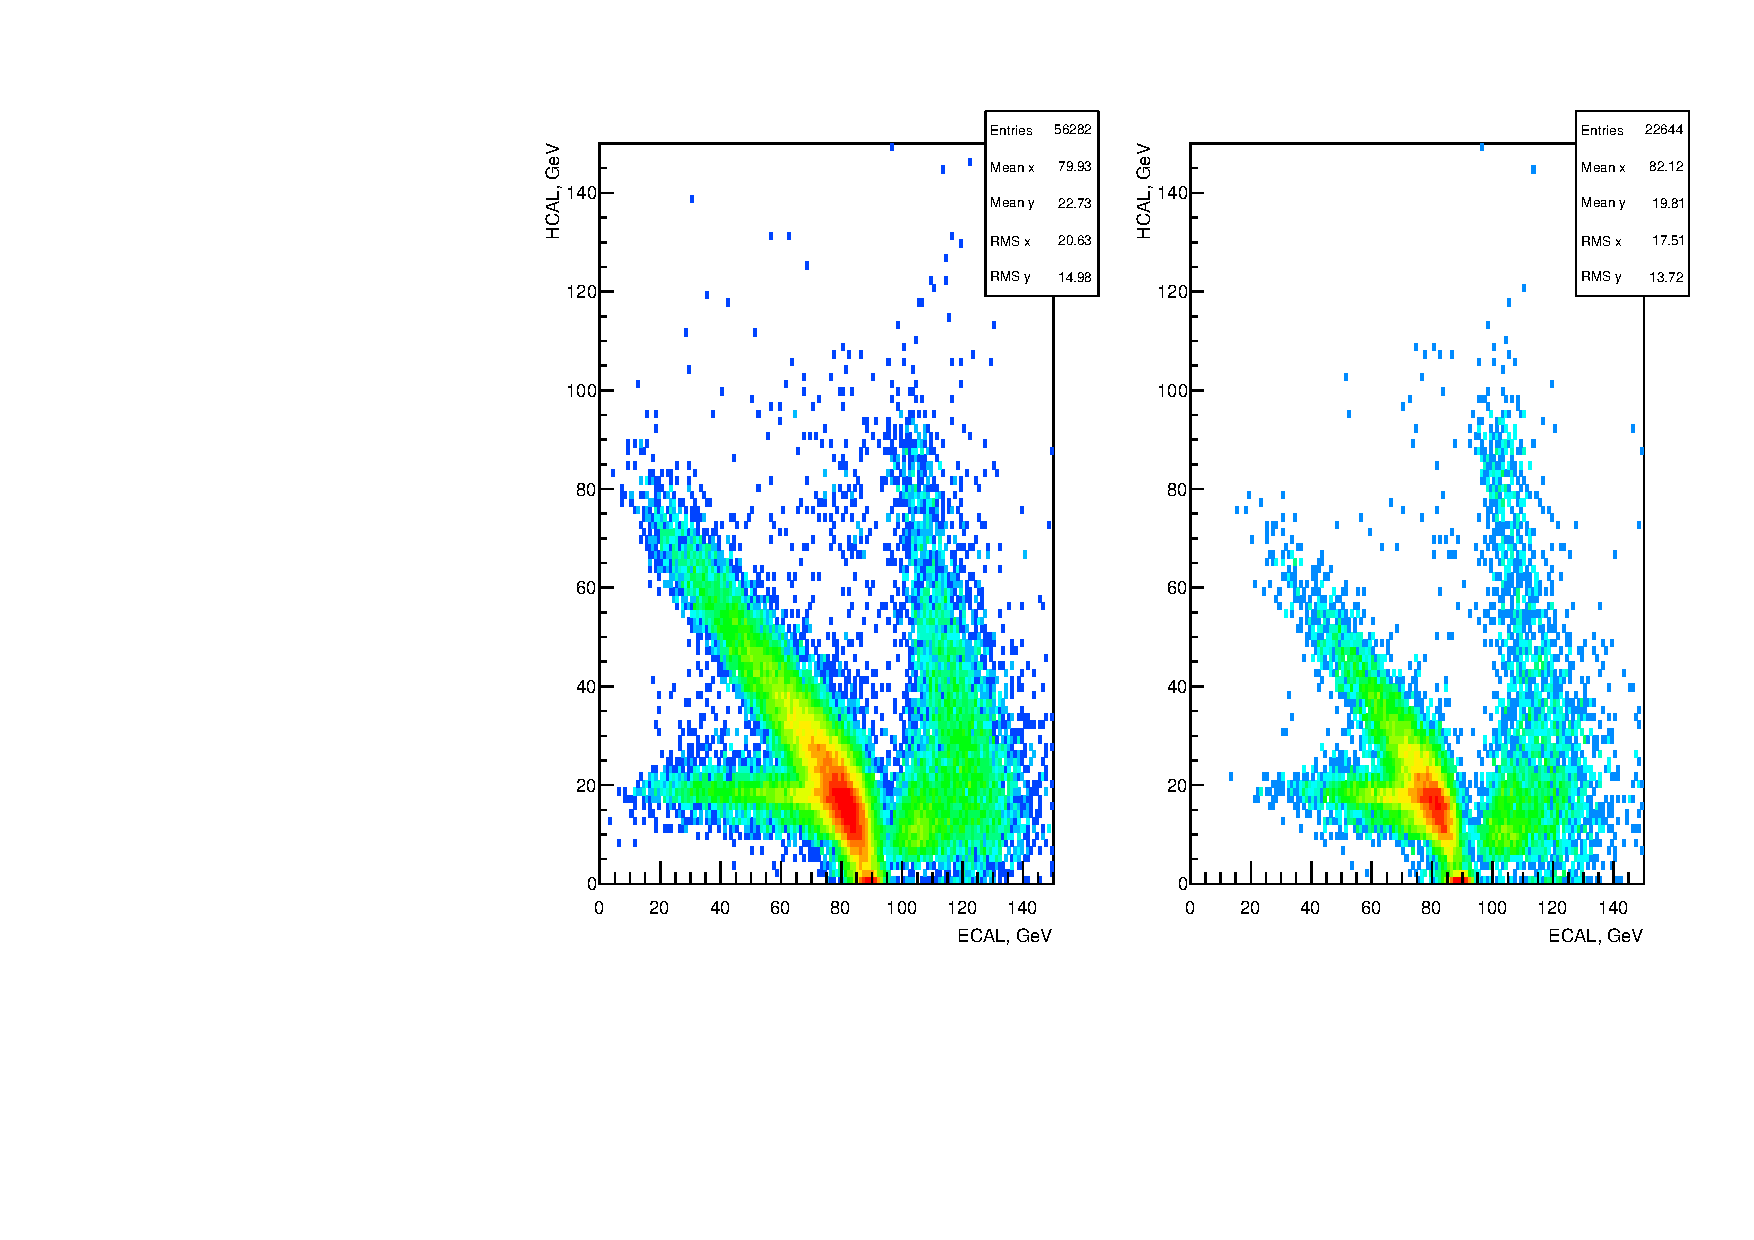
\includegraphics[width=0.95\textwidth,height=0.6\textwidth]{\pdirthree/ehcal_2441_comp.pdf}
  \end{center}
  \caption[ECAL vs HCAL energy deposit after a cut $\chi^2$ for different ECAL configurations]{ECAL vs HCAL after a cut $\chi^2<2$ in the physical run
    2441 with the $\chi^2$ calculated with the 9 central cells (left
    plot) and for all cells (right plot).}
  \label{fig:ehcal_comp}
\end{figure}



\section{Comparison with MC}
\label{ch3:sec:mc}
The same profiles described in the section above can be produced using
a 100 GeV electron simulation of the NA64 setup\cite{na64-simulation}. In
this section we will present some preliminary results for the
$\chi^2$-distribution produced using these profiles instead of the one
produced using the calibration runs.
\\
\\
The database produced using the MC simulation was applied both to the
same 100 GeV $e^-$ electron simulation, a 100 GeV $\pi^-$ simulation
and for the runs 2363 and 2204.  The first plot in
Fig.\ref{fig:chi_mc} shows that using the MC-database on the
simulation itself produces $\chi^{2}$-distributions consistent with
the one obtained in the previous section. However when the MC-database
is applied directly to the data an important shift is observed,
showing some incosistency between the two profiles, possibly caused by
the imperfect treatment of the pedestal and energy resolution and some
small mis-calibration of the cells.


\begin{figure}[h!]
  \begin{center}
    \includegraphics[width=0.95\textwidth,height=0.8\textwidth]{\pdirthree/chi_comp_mc.pdf}
  \end{center}
  \caption{$\chi^2$-distribution using shower profile database from a
    100 GeV electron MC-simulation over MC-simulation events (black)
    and over the electron run 2363 (red). The $\chi^2$-distribution
    was computed over all 36 ECAL cells.}
  \label{fig:chi_mc}
\end{figure}
\clearpage


More work is necessary to reach a good agreement between the
$\chi^{2}$-distributions, however separation between electrons and
hadrons is still achievable using the MC-database. 

We tested qualitatively the effect of a $\chi^{2}$-cut over the
ECAL vs HCAL plots produced for both the MC simulation
and the test runs considered in the previous section. For the
MC-simulation we used the same benchmark cut of the previous section
$\chi^2_{cut}$=2 , while for the runs 2363 and 2204 a benchmark cut of
$\chi^2_{cut}$=40 was used to take into account the shift in the
distribution observed. An additional cut was applied to the data to
remove the non-Gaussian tail of the beam since they were not covered
by the simulation
database, hence the statistic considered is a factor ~0.8 smaller.\\
\\
The bottom plot of Fig.\ref{fig:ehcal_elec} shows that the
contamination of hadron is removed when MC-database is used, so
the hadron shower still produces a significantly larger $\chi^{2}$
compared to the one of an electron shower. The efficiency
observed in the simulation is of ~0.98, slightly larger compared to the data. 
In both simulation and data we can observe that the characteristic
Di-muons events in the range [40,80] GeV in ECAL energy
deposition are accepted.
Fig.\ref{fig:ehcal_hadr} also shows the hadrons to be rejected in both
cases, with a rejection power of $\sim 5\times 10^{-3}$ measured in the
simulation. Also for both simulation and data we can observe that the
events surviving lie mostly in the diagonal $E_{ECAL}$+$E_{HCAL}$= 100
GeV (as could also be observed using a database built from calibration run like in Fig.\ref{fig:ehcal_comp}), while all the events where the shower has large angular spread are rejected.
\\
The main difference between the two plots concerns some events with very low energy deposited in the ECAL that are accepted in the data but not in the simulation. This would suggest that the ECAL cells are subject to some fluctuation that at low energy can sometime mimic the correct electromagnetic-shower signature. As stated in the previous section however for such low energy events the usage of the shower-profile algorithm should be avoided since all the shower will be completely contained in the cell 3x3.\\
% Finally the MC-database was applied to the physical run 2441 always
% with a benchmark cut $\chi^2_{cut}$=40.


\begin{figure}[h!]
  \begin{center}
    \includegraphics[width=0.95\textwidth,height=0.8\textwidth]{\pdirthree/ehcal_2363_chi_mc_2.pdf}
  \end{center}
  \caption{\textbf{Top}: ECAL vs HCAL before (left plot) and
    after (right plot) a cut
    $\chi^2<2$ in MC simulated 100 GeV electron events. \\
    \textbf{Bottom}: ECAL vs HCAL before (left plot) and after (right
    plot) a cut
    $\chi^2<40$ in the electron run 2363.\\
    The $\chi^2$ was computed using all ECAL cells with a shower
    profile database obtained from a 100 GeV $e^-$ MC-simulation. }
  \label{fig:ehcal_elec}
\end{figure}

\begin{figure}[h!]
  \begin{center}
    \includegraphics[width=0.95\textwidth,height=0.8\textwidth]{\pdirthree/ehcal_2204_chi_mc_2.pdf}
  \end{center}
  \caption{\textbf{Top}: ECAL vs HCAL before(left plot) and
    after(right plot) a cut
    $\chi^2<2$ in MC simulated 100 GeV $\pi^-$ events. \\
    \textbf{Bottom}: ECAL vs HCAL before (left plot) and after (right
    plot) a cut
    $\chi^2<40$ in the hadron run 2204.\\
    The $\chi^2$ was computed using all ECAL cells with a shower
    profile database obtained from a 100 GeV $e^-$ MC-simulation. }
  \label{fig:ehcal_hadr}
\end{figure}

\clearpage
\newpage

\subsection{Study of K$^0_S$ background in visible mode}
\label{ch3:sec:bkg-k0s}

\subsection{Study of neutral punch-through in the Calorimeters}
\label{ch3:sec:bkg-neutrals}

\section{Study of $\gamma + Z \rightarrow \mu^+ \mu^-$ events }
\label{ch3:sec:dimuons}

To validate the MC simulation and the tracking procedure required for this analysis, a pure sample of events containing the rare QED interaction $\emu$ has been studied. This class of events has many similarities to the $\DM$ ones, and they can be easily selected by requiring a double MIP signature in the HCAL modules. This procedure is described in detail in \cite{na64-prd}. The double tracks expected in the decay volume are then used to test the reliability of the tracking procedure in the setup.

To improve the quality of the MC, a realistic beam profile was extracted from the electron calibration runs. Hadrons in the sample were rejected by requiring an energy between 5 MeV and 100 MeV for both SRD counters. The beam profile is then recovered by fitting the XY position recorded by MM3,4 in Fig.\ref{fig:setup-vis-2018} with a 2D Gaussian. The two fits agree within 100 $\mu$m precision for both $\sigma_x \approx 4.13$ mm and $\sigma_y \approx 1.40$ mm. Fig.\ref{fig:dimuon:gemspectra} shows a comparison of the reconstructed hit-position between data and MC in $\emu$ events after the extracted beam profile is used in the simulation.

To further improve the agreement between data and MC several strategies were used. The limited spatial resolution of GEMs was taken into account by applying a smearing of 80 $\mu$m. This number was estimated by checking track residuals after selecting different GEMs triplets for the track reconstruction and comparing the reconstructed hit to the one predicted by the tracking procedure. To reproduce the single planes of the GEM, hits are separated in X-Y projections and knowledge on the original hit combination is no longer assumed. As the minimal hit separation between hits in GEM was conservatively estimated to be 1.75 mm, hits closer than this threshold were merged in the MC. This number was estimated using clusters recorded by the GEM detectors during electron run in 2017. The hits generated in this procedure are used as input for the same reconstruction algorithm used for the data.

The reconstruction chain works as follows:
\begin{enumerate}
\item Track candidates are defined by grouping hits where the angle between first and second GEM pair is smaller than 9 mrad.
\item Those candidates are reconstructed using a Kalman filter implemented with the Genfit library \cite{genfit}.
\item Vertex candidates are generated by grouping tracks pair with no common hits.
\item The exact position of the vertex is obtained by back-propagating the tracks at their point of minimum distance. Only vertices with a distance below 3 mm are considered for the analysis.
\end{enumerate}

\begin{figure}[tbh!]
  \begin{center}
    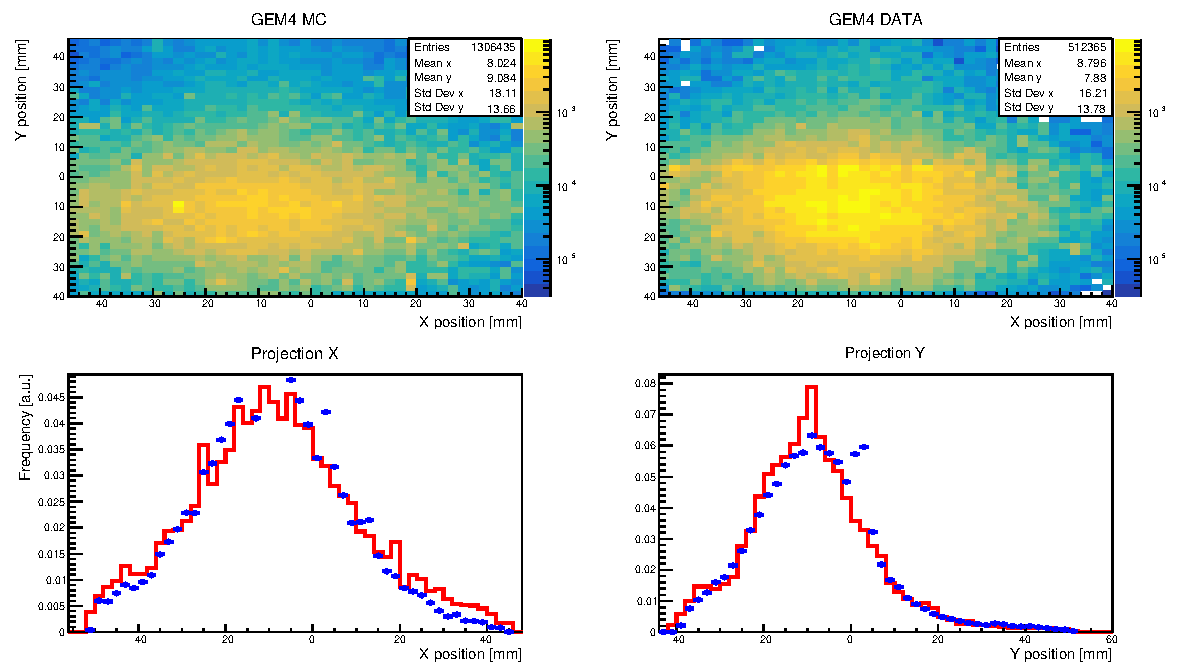
\includegraphics[scale=0.8]{\pdirthree/GEM4_rel.pdf}
  \end{center}

  \caption[Hit position of $\emu$ in GEM MC-DATA]{Hit position recorded in last GEM before ECAL for MC simulated (Red curve) and data (Blue dots) $\emu$ events.}
  \label{fig:dimuon:gemspectra}
\end{figure}
  

A dimuon sample was selected using all events collected during the visible mode 2018 run. The beam quality was improved by requiring a reconstructed momentum in the range between 140 and 160 GeV. The $\emu$ events leave a double-MIP signature in each HCAL module, thus a cut 2 GeV$<$ E$_{hcal} <$ 6.35 GeV is applied for the selection. Since an hardware trigger which selects only events with missing energy in the WCAL is used during the data taking, an additional cut $E_{WCAL} < 90$ GeV is applied to consider only such events in both simulation and data. This cut also selects a sample with kinematics closer to the one expected from a $\DM$ candidate. This makes the comparison with the MC more significant for our search. Scintillator counters also need to be compatible with a $\mu^+ \mu^-$ in the decay volume: an energy deposited of at least 1 MIP is required in the scintillator (S4) downstream the WCAL and at least 1.8 MIP in the Veto behind the ECAL. The less stringent cut on S4 is justified by its limited transverse dimension which makes it not suitable for a precise energy measurement.

Although these cuts mainly select dimuon generated from $e^-$ primaries, a contribution is also expected from the hadron contamination. The physical trigger employed in the experiment further increases such contribution, as the requirement of low energy deposit in the WCAL bias the beam composition to particles with high penetration power. To solve this issue, a cut on the SRD detector and on the WCAL pre-shower are used. These cuts are expected to reject hadrons and muons at a level $<10^{-5}$.

To cross-check that the contamination is correctly removed, an independent method based on the beam profile shape is used. The beam profile significantly differs between electrons and hadrons as the H4 beamline is tuned for selecting electrons in our search. Both profiles are recovered from the data using a calibration run of electron/hadron respectively. Using a  $\chi^2$-test the ratio between the two is estimated by mixing the two templates until the best agreement with the measured beam profile is reached. The result is summarized in Fig.\ref{fig:dimuon:profile}: the beam profile of dimuon-selection events is compared before and after the SRD criteria is applied. The fit shows a contamination of roughly 50\% in the original sample. After the cut the beam profile converges to the templates obtained in the $e^-$ calibration runs.

\begin{figure}[tbh!]
  \begin{center}
    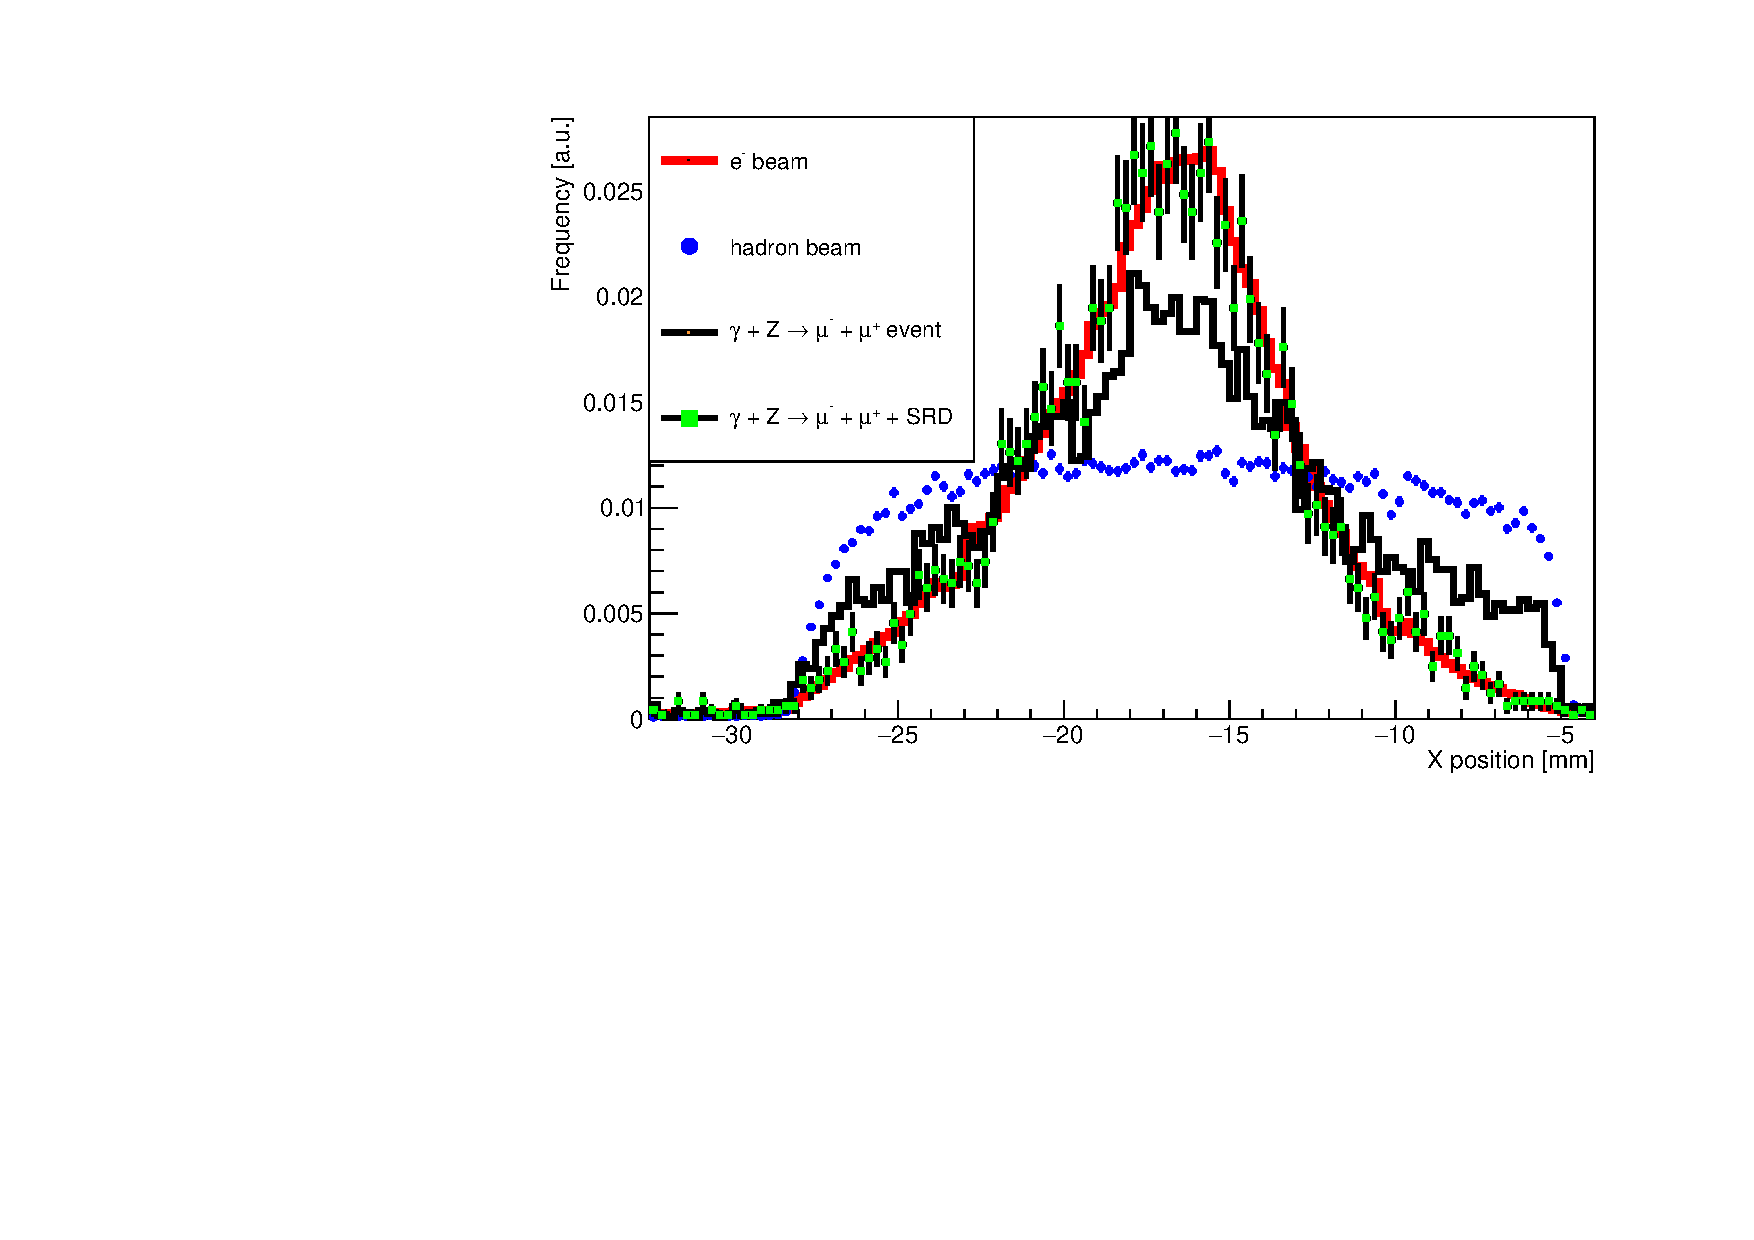
\includegraphics[scale=0.8]{\pdirthree/beamspot.pdf}
  \end{center}
  \caption[Beam profile with different cuts]{Beam profile recorded by the first Micromegas module upstream for hadron calibration run (blue dots), electron calibration run (red line), events selected with dimuons cuts from data collected with the physical trigger (black line) and those same events after SRD cut is applied (green square). Fits using the templates obtained from the calibration run show a level of contamination of $\sim$50\% in the dimuon sample. The contamination is completely removed after the SRD cut is applied.}
  \label{fig:dimuon:profile}
\end{figure}

%\subsection{Vertex and angle reconstruction}
%\label{ch3:sec:dimuons-reco}

\subsection{Signal yield correction}
\label{ch3:sec:dimuons-sig-corr}

To show that there are no significant differences in the tracking procedure between simulation and data the energy deposited in the WCAL was used as a figure of merit. If the tracking procedure affects differently data and MC, one would expect the agreement between the two distributions to diverge after cuts based on vertex reconstruction. Following the procedure described above, a number of vertex candidates are selected for the comparison. As the interaction $\emu$ will have their vertex inside the WCAL, only vertices compatible with this assumption are selected for the comparison. In practice, a vertex is accepted if its position lies within 3$\sigma$ of the expected WCAL position, where $\sigma$ was fitted using a Gaussian from the distribution of $\mu^- \mu^+$ pairs selected from the simulation. After the selection criteria, the energy deposited in the WCAL is compared between simulation and data for each event left (see Fig.\ref{fig:dimuon_en}). The energy deposit for data and simulation is in excellent agreement, proving that the tracking cuts do not bias the original sample.

\begin{figure}[tbh!]
  \begin{center}
    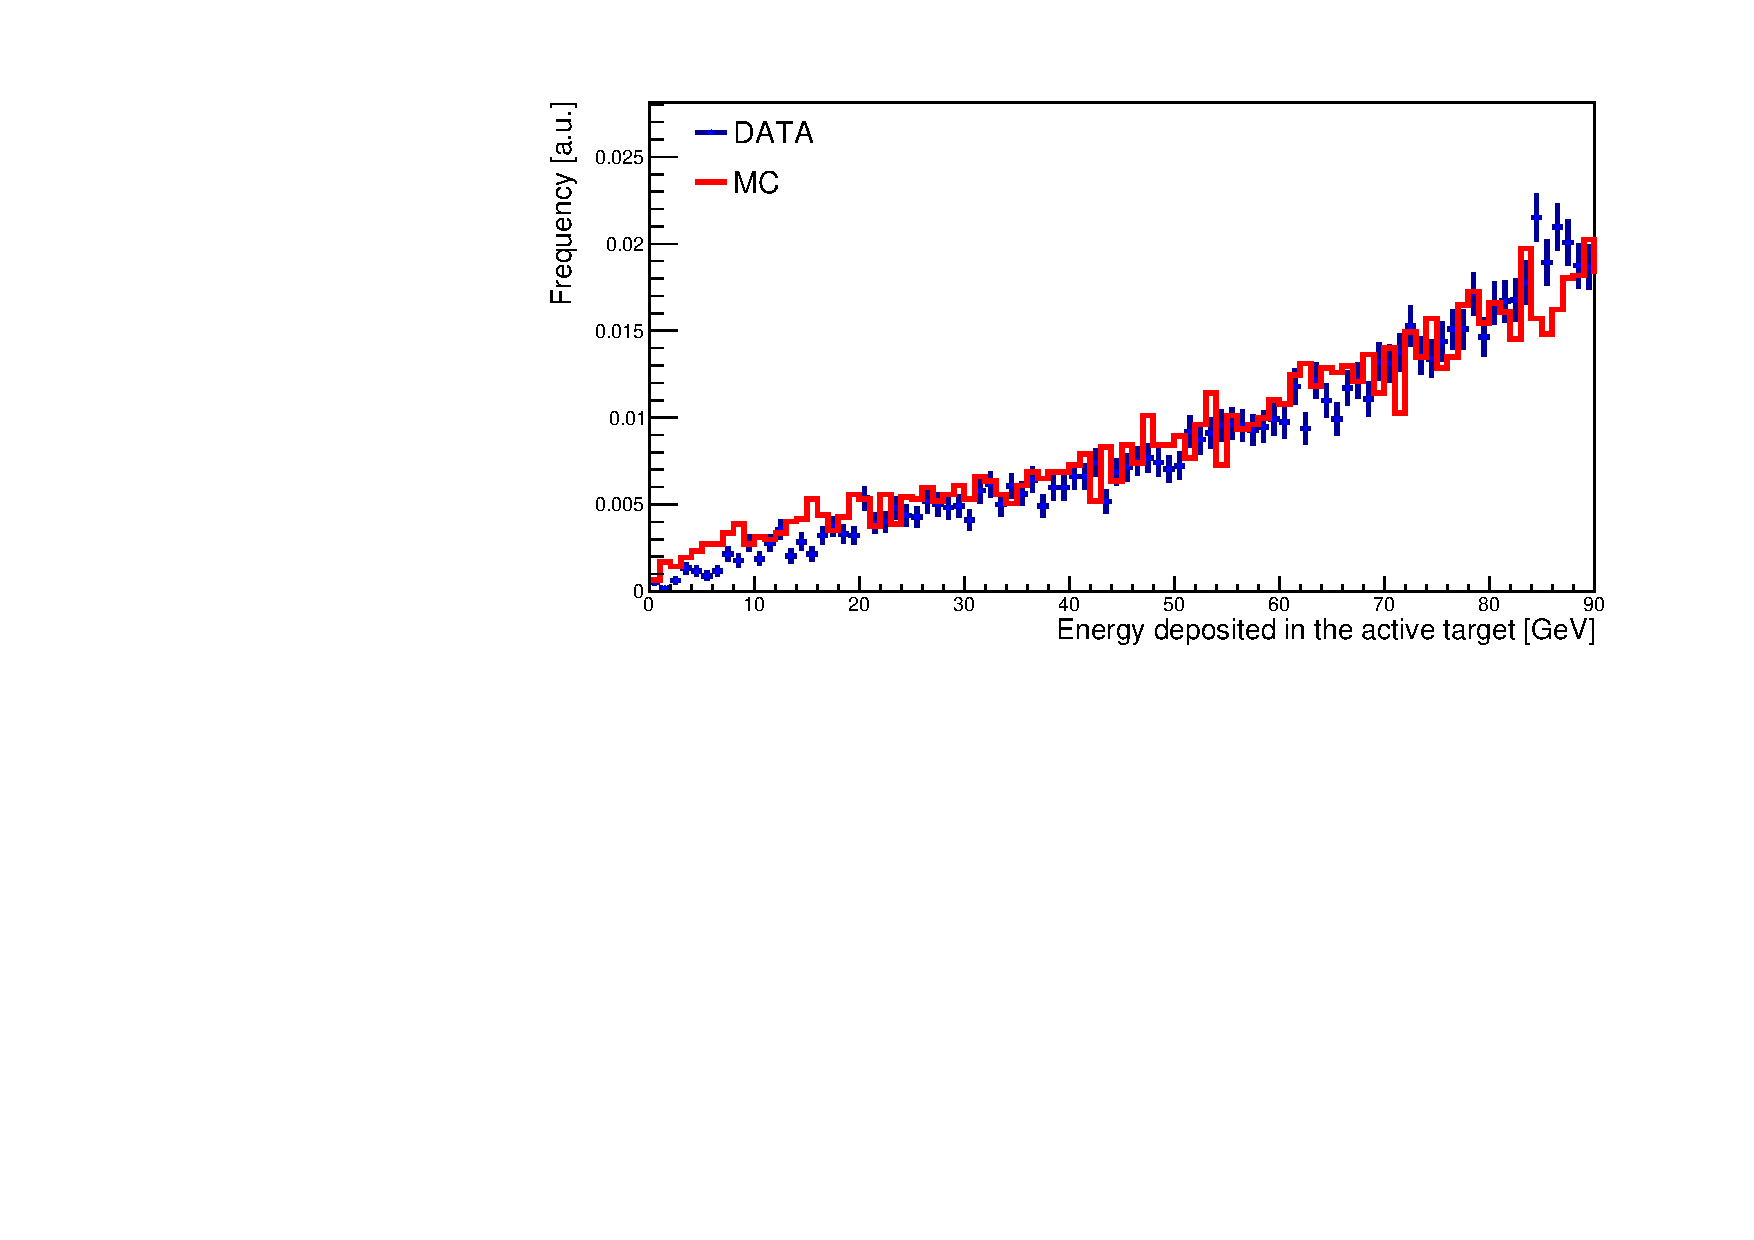
\includegraphics[scale=0.8]{\pdirthree/dimuon_en.pdf}    
  \end{center}
  \caption[$\emu$ MC-DATA comparison]{Energy deposit in the active dump (WCAL) after all selection criteria are applied in $\emu$ event. Data are drawn with blue dots, simulation is plotted with a red line. }
  \label{fig:dimuon_en}
\end{figure}

A lower efficiency is observed in the data compared to the Monte Carlo after applying the selection. The reasons for this are inefficiency of the GEM modules, fail of clusterization in some events and differences in the tracking procedure due to the simplifications used in the MC. The cuts applied to the sample are divided into four steps. First, at least two hits per GEM are required in the decay volume as a minimal condition for tracking. After that, events with a GEM module recording more than 5 hits are rejected as incompatible with a single $\emu$ vertex. The MC predicts 68\% of $\mu^+ \mu^-$ pair after these two cuts. This low acceptance is caused by the GEMs position optimized to resolve very close hits coming from the decay of $\DM$. These selection criteria do not depend on the track-fitting procedure but instead rely on the clusterization performed and the efficiency of the trackers. Tracking procedure is then applied to the events that survived the two first requirements. The reconstructed vertex position is required to be compatible with a vertex inside the dump. The number of events surviving the last requirement  is slightly smaller in the data. The disagreement between the ratio of good vertices reconstructed inside the decay volume is $<$1\%. A total factor of 0.77 is estimated as ratio between data and MC. This factor is used to correct the 2018 signal yield. A summary of the efficiency can be found in Table \ref{tab:dimuon:efficiencies}.

\begin{center}
\begin{table}
  %\centering
  \begin{tabular}{|l|c|c|c|}
    \hline
    cut & efficiency MC & efficiency Data & MC / DATA \\
    \hline
    \textbf{Hit} & & &\\
    \hline
    hits per GEM $\geq$ 2 & 0.68$\pm$0.1 & 0.58$\pm$0.1 & 0.85$\pm$0.1 \\
    hits per GEM $\leq$ 5 & 0.68$\pm$0.1 & 0.55$\pm$0.1 & 0.80$\pm$0.1 \\
    \hline
    \textbf{tracking} & & &\\
    \hline
    Vertex distance $\leq$ 3 mm & 0.63$\pm$0.1 & 0.49$\pm$0.1 & 0.77$\pm$0.1  \\
    Vertex in decay volume & 0.62$\pm$0.1 & 0.48$\pm$0.1 & \textbf{0.77$\pm$0.1}\\
    \hline
    
  \end{tabular}
  \caption[MC/DATA for the tracking procedure and vertex reconstruction]{Efficiency of cuts based on tracking criteria for a clean sample of simulated $\emu$ and dimuon selected from 2018 data. The efficiency presented in the table are cumulative, with the first cut applied being the one in the first row. First two cuts are based exclusively on information coming from the single GEM modules. Last two cuts are based on the tracking procedure.}
  \label{tab:dimuon:efficiencies}
\end{table}
\end{center}

\section{Selection criteria}
\label{ch3:sec:selection-criteria}

\subsection{Invisible mode}
\label{ch3:sec:selection-criteria-invis}

\subsection{Visible mode}
\label{ch3:sec:selection-criteria-vis}

\subsubsection{Analysis using Veto at the end of the dump}
\label{ch3:sec:vis-mode-veto}

\subsubsection{Mixed approach using tracking and Veto}
\label{ch3:sec:vis-mode-tracking}


The published analysis using the data collected in 2018 \cite{Banerjee:2019hmi} was based exclusively on the calorimeters and counters as described in Sec.\ref{ch2:sec:vismode}. The trackers after the decay volume were not used for the signal discrimination. Here we present a novel method which exploits them providing a boost in the signal yields while maintaining the background under control. Even though this analysis is not sensitive when the decay length of the $\DM$ is significantly smaller than the dimension of the dump, it has the advantage of being complementary to the calorimeter analysis. Moreover, it is a very important proof of principle to demonstrate the power of our tracking procedure.

While in a first approximation the $\DM$ is produced in the first few layers of the WCAL, it can also originate at a later stage of the em-shower. These events, which are typically rejected in the calorimeter analysis, are instead accepted in the new analysis presented here. First, an initial sample is selected in the same way described in Sec.\ref{ch2:sec:vismode} and detailed in \cite{Banerjee:2019hmi}. The final discrimination in the calorimeter analysis is based on the counter W2 placed at the end of the dump to reject the charged punch-through from the em-shower. This last cut is efficient if the $\DM$ is produced in the first few layers of the WCAL, but typically reject the event if the $\DM$ is produced at a later stage of the em-shower. The reason is that these events are accompanied by a long longitudinal development of the em-shower that leaves an energy deposit larger than the typical energy cut accepted in the calorimeter analysis. On the other hand, the low energy of the produced $\DM$ implies a larger angle between the decay products that can be resolved by the trackers. Combining these two concepts, one can see that the signal yield is characterized by two different topologies that can be easily distinguished by looking at the energy deposited in the ECAL (see Fig.\ref{fig:combined-analysis}).

Using this distinction, we divide all events that passed the initial selection criteria in two topologies based on the total energy deposited in the ECAL. The exact value of this threshold was selected to maximize the signal yield. The optimal value has a small dependence on the $\DM$ mass and coupling. A simple threshold of 75 GeV amounting to half of the initial beam energy was found to be robust for most of the interesting signal scenario. After the topology is decided, a final set of cuts is applied to discriminate between signal and background. In the case of high energy $\DM$, trackers do not have the capability of discriminate between single hits. An energy deposit smaller than 0.8 MIP is required in W2, and the presence of a decay after the dump is assessed by asking S4 to have an energy deposited larger than 1.5 MIP. On the other hand, if the energy deposited in the ECAL is smaller than 75 GeV, trackers are used instead as final discriminator. Two tracks in the decay volume are required with a reconstructed vertex within 3$\sigma$ from the WCAL and an angle smaller than 3 mrad. This different treatment leads to an increased efficiency to $\DM$ produced at a late stage of the shower as shown in Fig.\ref{fig:combined-analysis}. However, the smaller energy of the $\DM$ produced in this way has the effect of reducing the probability of the particle escaping the dump. For large coupling $\epsilon$ this suppression can be more than 2 orders of magnitude, making the boost of signal yield negligible. A summary of this boost for various interesting $\DM$ and $A'$ scenario is illustrated in Table \ref{tab:dm:efftable}. The values reported consider also a conservative correction factor of 0.77$\pm$0.1 that takes into account inefficiencies of the detectors and the reconstruction algorithm. This factor was evaluated using a data-driven method precisely outlined in Sec.\ref{ch3:sec:dimuons}. The conclusion of this study is that in the current setup trackers information do not improve the limit on the $\DM$ parameter space. This is because the boost in signal yield becomes negligible for $\epsilon \sim 6 \times 10^{-4}$, a value which is already excluded with 90\% confidence by our previous analysis.

\begin{figure}[tbh!]
  \centering
  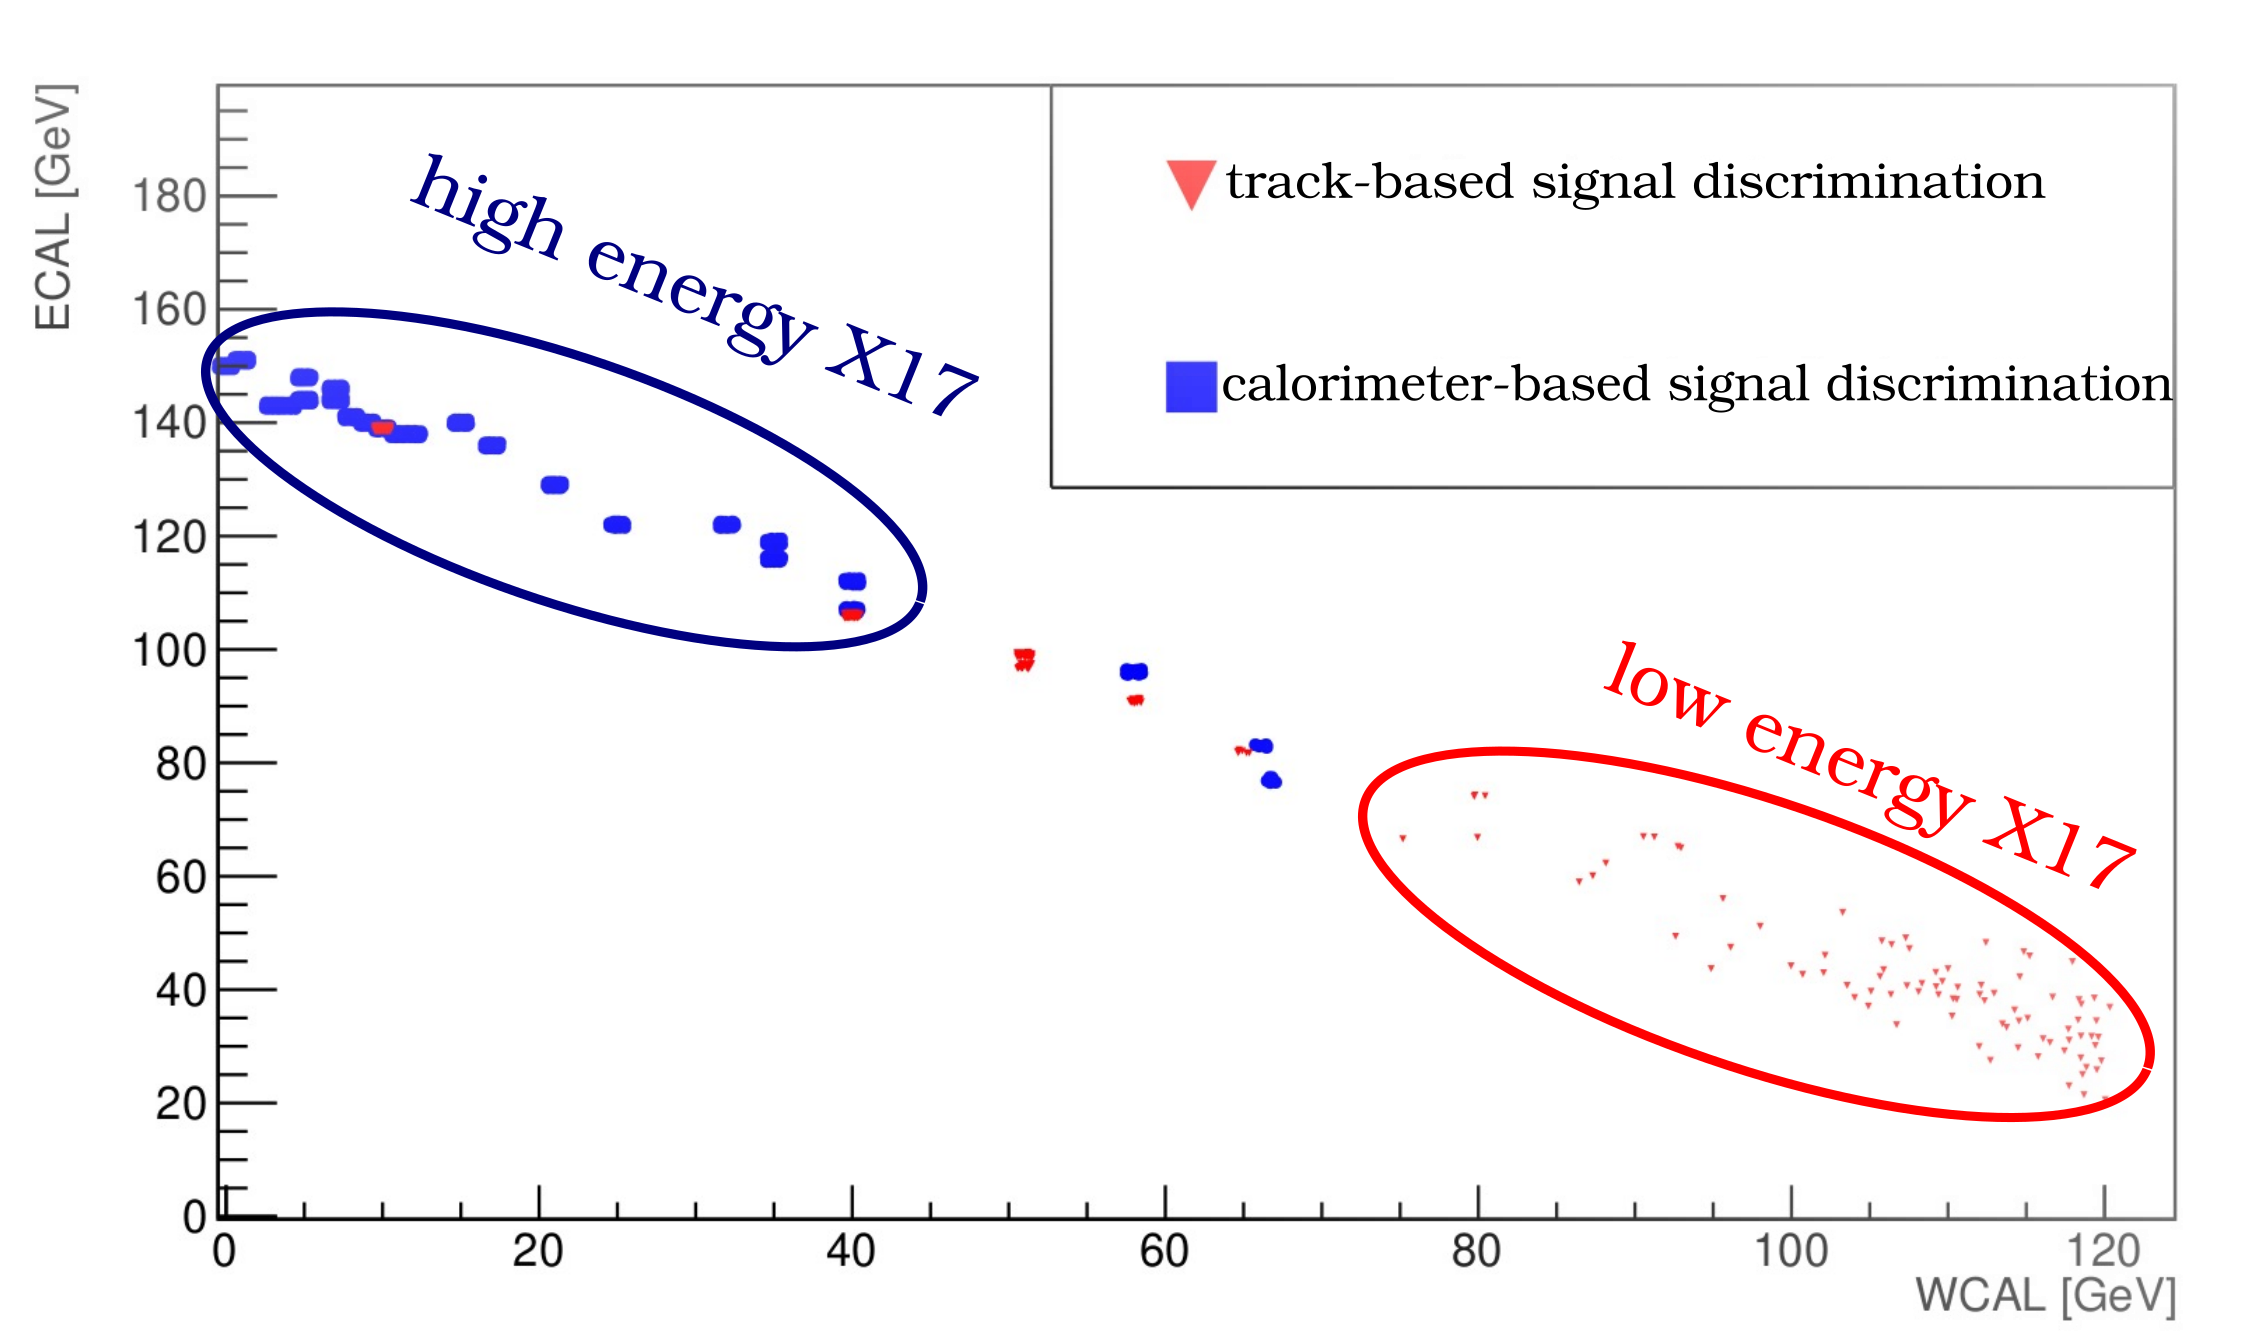
\includegraphics[scale=0.9]{\pdirthree/X17-separation-v2.png}
  \caption[Comparison of selected $\DM$ between calorimeter and tracking analysis]{$\DM$ simulated in the visible mode 2018 setup. Two different cuts are used to discriminate between two $\DM$ topologies. The first one is based on angle cut and vertex position using information from the 4 GEM stations installed in the decay volume and is very efficient on the $\DM$ produced at low energy (red triangle). The second one relies on the Veto placed at the end of the dump and is more efficient for the high energy population (blue square).}
  \label{fig:combined-analysis}
\end{figure}

\begin{center}
\begin{table}
  \centering
  \begin{tabular}{llr}
    \hline
    M$_{A'}$ [GeV]& $\epsilon$ & N$^{new}_{A'}$ / N$^{old}_{A'}$ \\    
    \hline
    0.005  & 0.004    & 1   \\    
    0.01   & 0.0015   & 1   \\    
    0.01   & 0.003    & 1   \\    
    0.0167 & 0.0001   & 1.22\\
    0.0167 & 0.00018  & 1.2 \\    
    0.0167 & 0.000316 & 1.2 \\
    0.0167 & 0.0006   & 1.01\\
    0.0167 & 0.0007   & 1   \\
    0.022  & 0.000316 & 1.22\\
    \hline    
  \end{tabular}
  \caption[ratio between signal events observed in tracker-analysis compared to calorimeter-only analysis]{N$^{new}_{A'}$ / N$^{old}_{A'}$ ratio between signal events observed in tracker-analysis compared to calorimeter-only analysis. The new analysis uses cuts based on GEM tracking detectors if the energy detected by the downstream ECAL is below 75 GeV.}
  \label{tab:dm:efftable}
\end{table}
\end{center}



%%% Local Variables:
%%% mode: latex
%%% TeX-master: "../PhDthesis"
%%% End:
